
\documentclass[12pt,a4paper,oneside]{book}

\makeatletter
\newcommand\thefontsize[1]{{}}
\makeatother
\usepackage[utf8]{inputenc}
\usepackage{enumitem}
\usepackage{varwidth}
\usepackage{graphicx}
\usepackage{caption}

\usepackage[top=2.5cm, bottom=3cm, left=2.5cm, right=2.5cm]{geometry}
\usepackage[utf8]{inputenc}
\usepackage[titletoc,title]{appendix}
\usepackage[linewidth=1pt]{mdframed}
\usepackage{framed}
\usepackage{listings}
\usepackage{smartdiagram}
\usepackage{smartdiagram}
\usepackage{varwidth}
\usepackage{amsmath}

\usepackage[linesnumbered,ruled,vlined]{algorithm2e}
\usesmartdiagramlibrary{additions}
\lstdefinestyle{customc}{
	belowcaptionskip=1\baselineskip,
	breaklines=true,
	frame=L,
	xleftmargin=\parindent,
	language=C,
	showstringspaces=false,
	basicstyle=\footnotesize\ttfamily,
	keywordstyle=\bfseries\color{green!40!black},
	commentstyle=\itshape\color{purple!40!black},
	identifierstyle=\color{blue},
	stringstyle=\color{orange},
}


\lstset{escapechar=@,style=customc}

\lstset{
	literate=%
	{à}{{\'a}}1
	{í}{{\'i}}1
	{é}{{\'e}}1
	{è}{{\`e}}1
	{ý}{{\'y}}1
	{ú}{{\'u}}1
	{ó}{{\'o}}1
	{ě}{{\v{e}}}1
	{š}{{\v{s}}}1
	{č}{{\v{c}}}1
	{ř}{{\v{r}}}1
	{ž}{{\v{z}}}1
	{ď}{{\v{d}}}1
	{ť}{{\v{t}}}1
	{ň}{{\v{n}}}1
	{ů}{{\r{u}}}1
	{Á}{{\'A}}1
	{Í}{{\'I}}1
	{É}{{\'E}}1
	{Ý}{{\'Y}}1
	{Ú}{{\'U}}1
	{Ó}{{\'O}}1
	{Ě}{{\v{E}}}1
	{Š}{{\v{S}}}1
	{Č}{{\v{C}}}1
	{Ř}{{\v{R}}}1
	{Ž}{{\v{Z}}}1
	{Ď}{{\v{D}}}1
	{Ť}{{\v{T}}}1
	{Ň}{{\v{N}}}1
	{Ů}{{\r{U}}}1
}
\usepackage{booktabs,makecell,tabularx}

\renewcommand\theadfont{\small}
\newcolumntype{L}{>{\raggedright\arraybackslash}X}
\usepackage{siunitx}
\usepackage{adjustbox}
\usepackage{array,booktabs}

\usepackage{graphicx}
\usepackage{epstopdf}

%\newcolumntype{C}[1]{>{\centering\arraybackslash}p{#1}}
\usepackage{algorithm}% http://ctan.org/pkg/algorithms
\usepackage{algpseudocode}% http://ctan.org/pkg/algorithmicx
\usepackage{amsmath}
\begin{document}
	
	\def\reportnumber{}
	\def\reporttitle{Implémentation de Techniques de Data-Mining }
	%----------------------------------------------------------------------------------------
%	TITLE PAGE
%----------------------------------------------------------------------------------------

\begin{titlepage} % Suppresses displaying the page number on the title page and the subsequent page counts as page 1
	\newcommand{\HRule}{\rule{\linewidth}{0.5mm}} % Defines a new command for horizontal lines, change thickness here
	
	\center % Centre everything on the page
	
	%------------------------------------------------
	%	Headings
	%------------------------------------------------
	
	\baselineskip=2\baselineskip 
	\textsc{\LARGE Université des Sciences et de la Technologie Houari Boumediene}%\\[1cm] % Main heading such as the name of your university/college

	%------------------------------------------------
	%	Logo
	%------------------------------------------------
	
	%\vfill\vfill
	\vfill
	
\includegraphics[width=0.3\textwidth]{USTHB_Logo.png}\\[1cm] % Include a department/university logo - this will require the graphicx package
	 
	%----------------------------------------------------------------------------------------
	
	\textsc{\Large Data Mining }\\[0.5cm] % Major heading such as course name
	%\textsc{\large Minor Heading}\\[0.5cm] % Minor heading such as course title
	
	%------------------------------------------------
	%	Title
	%------------------------------------------------
	
	\HRule\\[0.4cm]
	\baselineskip=1.2\baselineskip 
	{\huge\bfseries Résumé du livre "Data Mining
		Concepts and Techniques"\textdegree  \reportnumber \\ \reporttitle}\\[0.4cm] % Title of your document
	
	\HRule\\[1.5cm]
	
	%------------------------------------------------
	%	Author(s)
	%------------------------------------------------
	
	\begin{minipage}{0.4\textwidth}
		\begin{flushleft}
			\large
			\textit{Rédaction:}\\
			MOULAI \textsc{Hassina Safaa}\\ % Your name
			Matricule : 201400007564\\ 
			
			HOUACINE \textsc{Naila Aziza}\\ % Your name
			Matricule : 201400007594\\ 
			
			M2 SII Groupe:3\\
			
		\end{flushleft}
	\end{minipage}
	~
	\begin{minipage}{0.4\textwidth}
		\begin{flushright}
			\large
			\textit{Professeur}\\
			Mme. BABA ALI  % Supervisor's name
		\end{flushright}
	\end{minipage}
	
	%------------------------------------------------
	%	Date
	%------------------------------------------------
	
	\vfill\vfill\vfill % Position the date 3/4 down the remaining page
	
	{\large\today} % Date, change the \today to a set date if you want to be precise
	
	
	\vfill % Push the date up 1/4 of the remaining page
	
\end{titlepage}
	
	
	\sffamily
	
	\setcounter{tocdepth}{2}
	\tableofcontents
	\listoffigures
	\newpage
	
	\chapter*{Introduction [1,2] }
	
	La quantité de données collectées quotidiennement ne cessent de croitre, celle-ci étant considérée comme une mine de connaissance qui n'attend qu'a être exploité. il en va de soit qu'analyser ces données
	est un besoin important. l'exploration de données (ou Data-Mining) peut répondre à ce besoin tel que:
	
	L'exploration de données permet de trouver des informations précieuses cachées dans de grands volumes de données.
	
	L'exploration de données est l'analyse des données et l'utilisation de techniques informatiques pour trouver des modèles et des régularités dans des ensembles de données (DataSet).
	
	Le processus de Data-Mining est responsable de la recherche des modèles en identifiant les règles et fonctionnalités sous-jacentes des données.
	
	Il est possible d'extraire des schémas jusqu'alors inconnus ou si évidents que personne ne les avait remarqués auparavant.
	
	
	Le Data-Mining repose sur quelques technologies indispensables dont: l'algorithmique (et structure de données), les Statistiques, l'apprentissage automatique, Systèmes de bases de données et entrepôts de données ainsi que la recherche d'information...\\
	En utilisant ces technologies le processus de Data-Mining passe par plusieurs étapes, celles-ci peuvent ce résumer comme suit:
	\begin{enumerate}
		
		
		\item \textbf{Pré-traitement des données}: c'est à dire :
		Traitement de valeurs manquantes,
		Nettoyage des données,
		Normalisation de données,
		Réduction de données,
		Discrétisation, ...
		
		
		\item \textbf{Création de modèle de données}: application des outils intelligents de Data-Mining pour extraire des connaissances à partir de données, Pour cela le nombre d'outils et de techniques existants est suffisamment conséquent pour couvrir tous les types de problèmes, citons: l'extraction d'items fréquents et associations minières, classification supervisée : Arbres de décision, K-nn, Classification bayésienne, ..., classification non supervisée et clustering: K-means, K-medoid, Agnes, Dbscan, ...
		
		
		\item \textbf{Tester le modèle}: les performances du modèle (par exemple, le rappel, la précision, l'exhaustivité, ...) sont testées sur des données indépendantes (non utilisées pour créer le modèle).
		
		
		\item \textbf{Interprétation et évaluation}: En commençant par visualiser les résultats obtenus, Nous serons en mesure d'en extraire des observations et conclusions après les expérimentations, aussi nous serons en mesure d'apporter des améliorations aux techniques testées.
		
		
		
		
	\end{enumerate}
	\newpage
	
	\chapter{Algorithme d'extraction d'items fréquents et associations minières}
	\section{Introduction}
	
	Les algorithmes d'extraction d'items fréquents et règles d'associations sont très largement exploités car en plus de leur efficacité, nombreux sont les domaines d'application, nous citons à titre d'exemple:
	\begin{enumerate}
		
		
		\item Analyse des logs web sur un serveur web afin de découvrir le comportement utilisateur, et ainsi adapter et personnaliser le site à leurs attentes. [3]
		
		\item Le panier de la ménagère qui décrit l'ensemble des achats au supermarché, tel que nous pouvons en extraire les produits qui se vendent ensemble, et ainsi décider de leur disposition dans les étagères selon le but du super marché. [3]\\
		
		Ou alors de choisi les réductions et promotions à effectuer sur des ensembles de produits.
		
		\item ... etc.
		
	\end{enumerate}
	
	Pour cela diverse techniques et algorithmes existent, dont les plus populaires et plus utilisés : \textbf{Apriori}, \textbf{FP-Growth} et \textbf{Eclat}\\
	Dans ce qui suit nous allons nous interesser aux deux algorithmes \textbf{Apriori} et \textbf{FP-Growth}.
	

	\section{Apriori}
	\subsection{Principe de fonctionnement}
	L'algorithme \textbf{Apriori} à été conçu en 1994, par \textit{Rakesh Agrawal} et \textit{Ramakrishnan Sikrant}, dans le domaine de l'apprentissage des règles d'association.[2]
	
	Apriori emploie une approche itérative  tel que chaque k-itemsets est utilisé pour explorer les (k+1)-itemsets.\\
	\textbf{ }\\
	\textbf{Complexité:}\\
	La complexité Temporelle de \textbf{Apriori} est cubique,  en \textbf{\textit{O($(n * m)^2 * k$)}}.\\
\textbf{ }\\
Car pour la détermination de l'ensemble courant des candidats : la jointure se fait en O($|L|^2$ ). Mais comme $|L|$ est égal au maximum à (n * m), la complexité de la jointure est O($(n * m)^2$ ).\\
\textbf{ }\\	
La complexité Spatial  de \textbf{Apriori} est en \textbf{\textit{O($n^2$)}}.\\
	
		Avec: 
		
		$n$ : nombre d'items distincts du DataSet transactionnel.
		
		$m$ : nombre de transactions.
		
		
		$k$ : nombre d'itération (qui correspond aussi au max k-itemset).	
	
	
	\subsection{Structures de données}
	Afin de bien résoudre notre problème qui est d'appliquer l'algorithme apriori sur un dataset transactionnel et d'extraire les items fréquents il a fallu modéliser et structurer nos données .
	
	\subsubsection{Transaction}
	une transaction sera modéliser comme suit:
	\begin{itemize}
		\item  \textbf{idtransaction:} qui est le numéro de la transaction
	\end{itemize}
	\subsubsection{SetofTransaction}
	\begin{itemize}
		\item  \textbf{set\_T}(ensemble de transaction) qui est HashMap$<$Transaction, ArrayList$<$item$>>$
	\end{itemize}
	une HashMap est un dictionnaire qui prend comme clé des  transactions et comme valeurs un ensemble d'items (itemset)
	
	\subsubsection{Item}
	\begin{itemize}
		\item \textbf{Itemname} :  est le nom de l'item exemple : i1,i2...
		
	\end{itemize}
	\subsubsection{Itemset}
	\begin{itemize}
		\item \textbf{ items} : qui est un hashset d'item hashset est un ensemble d'éléments ( un élément n'apparait qu'une seule fois sans répétition)
		\item\textbf{ frequence} : qui est la fréquence (type integer) de l'itemset
	\end{itemize}
	\subsubsection{SetItemset}
	
	
	\begin{itemize}
		\item\textbf{ set\_itemset :} qui est un ensemble d
	\end{itemize}
	
	\subsection{Pseudo-code}
	
	
	
	\begin{algorithm}[H]
		\DontPrintSemicolon
		\KwIn{D,base de données de transations ,support minimum}
		\KwOut{L, itemset fréquent dans D}
		L1= find frequent 1-itemsets(D);
		
		\For{$k \gets 2; L_{k-1} != \emptyset;k++$}{
			$C_{k} \gets apriori_gen(L_{k-1})$\;
			
			\For {$transaction$ $t$ $ \in D$}{
				
				scan D for counts\\
				% The "l" before the If makes it so it does not expand to a second line
				$C_{t}$=subset($C_{k}$,t); génerer les subsets de t qui sont candidats
				
				
				\For {candidate $c$ $\in$ $C_{t}$}{
					
					c.count++;
					
					$L_{k}$={ $c \in C_{k}$ , c.count$>$support minimum}}
				
				
			}
			
		}
		\Return{$L= \bigcup\limits_{k} L_{k}$}\;
		\caption{{\sc APRIORI}}
		\label{algo:duplicate1}
	\end{algorithm}
	\subsection{Explication}
	les differentes étapes :
	
	\begin{enumerate}
		\item Exploration de la base de données pour avoir le support de chaque 1-itemset (ensemble d'un seul item).
		\item Comparer le support(fréquence) avec le\textbf{ min\_supp} .
		\item  Supprimer les 1-itemsets ayant un support inférieur au \textbf{ min\_supp} génerer alors $L1$.
		\item Faire une jointure de $L_{k-1}$ avec $L_{k-1}$  pour générer les ensembles de candidate k-itemsets.
		\item Verifier la propriété APRIORI  pour élaguer les k-itemsets qui ne sont pas fréquents.
		\item Exploration de la base de données pour avoir le support de chaque candidate k-itemset vérifiant la propriété apriori.
		\item Comparer le support de chaque candidate k-itemset avec \textbf{ min\_supp}
		\item Garder que l'ensemble des k-itemsets vérifiant la condition de  \textbf{ min\_supp} et on aura ainsi $L_{k}$
		\item si $L_{k}$ est vide alors pour chaque frequent itemset 1 générer les subsets non vide de 1, et pour chaque s subsets non vide de 1, écrire la règle "s implique(1-s)" si la confidence C de la règle "s implique 1-s" satisfait le \textbf{support min de confiance }
		\item sinon aller à 4
	\end{enumerate}
	
	
	
	
	
	\newpage
	
	\section{Fp-growth}
	\subsection{Principe de fonctionnement}
	L'algorithme \textbf{Fp-growth} dont \textbf{Han} (2000) est le créateur, est une méthode efficace et évolutive pour l'exploitation minière. \\
	Cet Algorithme utilise une structure d'arborescence de préfixes étendue pour le stockage d'informations compressées et cruciales sur les modèles fréquents nommés arborescence de modèles fréquents \textbf{FP-Tree}.[2]\\
	
	FP-Growth construit l'arbre FP-Tree à partir des transactions données dans le dataset à traiter, puis filtre les ItemSets vérifiant le support minimal, ensuite de manière incrémentale en parcourant le FP-Tree il construit pour chaque Item ce qu'on appelle \textit{Conditional Pattern Base} c'est à dire les motifs conditionnelles de base (les chemins vers l'item) qui servirons à leurs tour dans la génération des \textit{Conditional FP-tree} ceux-ci préfixés par leur Item correspondant, formeront les \textbf{motifs fréquents} recherchés.[2] 
	
	
	\textbf{ }\\
	\textbf{Complexité:}\\
	La complexité Temporelle de \textbf{FP-Growth} est Polynomial,  en \textbf{\textit{O($n^2$)}}.\\
	La complexité Spatiale  de \textbf{FP-Growth} est en \textbf{\textit{O($n^2$)}}.
	
	
	Avec: $n$ : nombre d'items distincts du DataSet transactionnel.
	
	\subsection{Structures de données}
	
	\subsection*{Item}
	Nous avons défini la structure de \textbf{Item}, celle-ci représente un item d'une transaction, tel qu'elle est composée de 2 attributs:
	\begin{itemize}
		\item[$\bullet$] \textbf{itemName:}chaine de caractère représentant le nom de l'item (\textit{exemple: "i1"})
		\item[$\bullet$] \textbf{Support:} entier (int), support de cet item c'est à dire ca fréquence dans le Dataset.
	\end{itemize}
	
	
	\subsection*{ItemSet}
	Il s'agit d'un ensemble d'Items ayant un support, ainsi un ItemSet est composé des 2 attributs suivants:
	\begin{itemize}
		\item[$\bullet$] \textbf{Items:} Liste d'Item qui peut correspondre à une branche de la FP-Tree.
		\item[$\bullet$] \textbf{Support:} il s'agit du support minimal des Item de la liste.
	\end{itemize}
	
	
	
	\subsection*{Tree}
	Il s'agit du FP-Tree, l'arbre permettant la représentation compressée des transactions du dataset, tel que chaque nœud possède les 3 éléments suivants:
	\begin{itemize}
		\item[$\bullet$] \textbf{Item:} l'item du nœud courant.
		\item[$\bullet$] \textbf{Children:} la liste les fils du noeud courant, qui est une liste de nœuds de la même structure \textit{Tree}.
		\item[$\bullet$] \textbf{Dad:} Le nœud de même structure \textit{Tree}, qui le parent du nœud courant. 
	\end{itemize}
	
	
	\subsection*{Rule}
	Cette structure représente une règle d'association,
	celle-ci ayant la forme suivante:
	\begin{center}
		\textbf{Condition $\Rightarrow$  Conclusion : Confiance = XXX\% }
	\end{center}
	Nous avons alors représenté chaque règle avec les 3 éléments suivants:
	\begin{itemize}
		\item[$\bullet$] \textbf{Condition:} un ItemSet représentant la partie gauche de la règle d'association.
		\item[$\bullet$] \textbf{Conclusion:} un ItemSet représentant la partie droite de la règle d'association.
		\item[$\bullet$] \textbf{Confiance:} (double) Degré de confiance de cette règle (en \%).
	\end{itemize}
	
	
	\subsection*{fp-growth}
	Il s'agit d'une instance pour l'exécution de FP-Growth, telle que les éléments de base nécessaires pour cela y sont structurés comme suit:
	\begin{itemize}
		\item[$\bullet$] \textbf{DataSet:} le dataset contenant les transactions/items dont nous souhaitons étudier les motifs fréquents.
		\item[$\bullet$] \textbf{fp-tree:} l'arbre utiliser pour la représentation compressé du dataset.
		\item[$\bullet$] \textbf{Support\_min:} support minimal à prendre en compte lors de la recherche d'ItemSet fréquents.
		\item[$\bullet$] \textbf{Confidence\_min:} la confiance minimal à prendre en compte pour valider une règle.
		
	\end{itemize}
	
	
	\subsection{Pseudo-code}
	\begin{algorithm}[H]
		\DontPrintSemicolon
		\KwIn{D:base de données de transations ,$Supp_{min}$ :support minimum }
		\KwOut{L: itemset fréquent dans D}
		
		L= find frequent 1-itemsets(D);
		
		//Create the root of an FP-tree, and label it as “null.”
		
		$FP_{tree}$ = $\{null\}$
		
		\ForEach{Trans in D}
		{
			Sort Items of (Trans) according to the order of (L)\\
			\ForEach{Item in Trans}{
				//$FP_{tree}$ is the first element\\
				//P is the remaining list\\
				Insert\_tree([$FP_{tree}|$P], Item)
			}
		}
		
		L = FP-growth-Const(${FP}_{tree}, null$)
		
		\Return{$L$}\;
		\caption{\sc FP-Growth}
	\end{algorithm}
	
	
	
	
	\begin{algorithm}[H]
		\SetAlgoLined
		\DontPrintSemicolon
		\textbf{Procedure : Insert\_tree([p|P], Item)}\;
		
		\If{Item.has\_a\_child(N) \textbf{And} N.item-name = $p$.item-name}
		{
			N.freq ++
		}
		\Else{
			Create\_Node(N)\\
			N.freq = 1\\
			Link\_To\_Parent(Item, N)
		}
		\If{P.empty() == False}
		{insert\_tree(P, N)}
		
		
		\Return $P$\;
		\caption{\sc Procedure Insert\_tree }
	\end{algorithm}
	
	
	
	\begin{algorithm}[H]
		\DontPrintSemicolon
		\textbf{procedure FP\_growth-Const(Tree, $\alpha$)}
		
		\If{Tree contains a single path P}
		{
			\ForEach{combination $\beta$ of the nodes in the path P}{
				generate pattern $\beta \cup \alpha$  with support\_count = minimum support count of nodes in $\beta$;
			}
		}	
		\Else{ 
			\ForEach{ $a_{i}$ in Q /*the header of Tree*/} 
			{
				generate pattern $\beta = a_{i} \cup \alpha$ with support\_count = $a_{i}$.support\_count
				
				construct $\beta$ conditional pattern base and then $\beta$  conditional FP\_tree $Tree_{\beta}$
				
				\If{$Tree_{\beta}$ = $\emptyset$} {
					FP\_growth($Tree_{\beta}$ , $\beta$) 
				}
				set(Q) is the set of patterns generated
				
			}
		}
		\Return{$\alpha$}\;
		\caption{\sc Procedure FP-Growth-Const}
	\end{algorithm}
	
	\subsection{Explication}
	Les différentes étapes :
	
	\begin{enumerate}
		\item Exploration de la base de données pour avoir le support de chaque 1-itemset (ensemble d'un seul item).
		\item Comparer le support(fréquence) avec le\textbf{ min\_supp} .
		\item  Supprimer les 1-itemsets ayant un support inférieur au \textbf{ min\_supp} , et ordonner les autres Items dans l'ordre décroissant de nombre de support, générer alors $L$.
		\item Initialiser notre $FB_{Tree}$ a $null$
		\item Ordonner les Item de chaque transaction selon l'ordre obtenu dans $L$
		\item Construction de $FB_{Tree}$ de manière itérative:
		
		Pour chaque Transaction insérer les items la formant dans le $FB_{Tree}$
		
		tel que: soit on ajoute un nœud (si celui-ci n'existe pas), soit on incrémente la fréquence du nœud (dans le cas contraire).
		
		\item Pour chaque Item de $L$ toujours dans l'ordre décroissant de fréquence et en utilisant une stratégie de profondeur d'abord:
		
		On détermine l'arbre de cet Item (tous les chemins allant de la racine $\{\}$ à cet Item)
		
		\item si l'on trouve un seul chemin P constitué d'un ensemble d'Items, alors on génère toutes les combinaisons  $\beta$ de ces Items.
		
		\item On récupère les combinaisons $\beta$ ayant un support $\geq$ \textbf{ min\_supp} que l'on ajoute à notre liste de motifs fréquents $\alpha \cup \beta$.
		
		\item Sinon (plusieurs chemins) alors, faire l'union des chemins, tel que pour chaque item nous lui donnerons comme support la somme des supports des itemSet auxquels il appartient.
		
		\item Supprimer les motifs de support $<$ \textbf{ min\_supp} 
		
		\item Construire la base de motifs conditionnels à partir de $\beta$  
		
		\item une fois toutes les combinaisons récupérées, on fait un appel récursif de FP-Growth avec la nouvelle liste $\beta$ (retour à 8)
	\end{enumerate}
	
	\newpage
	
	\section{Comparaison et remarques}
	\subsection{DataSet}
	Le DataSet utilisé pour nos expérimentation est un DataSet publique et reconnu, disponible sur le site : \textbf{UCI}. [4]\\
	Celui-ci est un dataset transactionnel qui contient toutes les transactions intervenues et enregistrées entre le 01/12/2010 et le 09/12/2011 pour un détaillant en ligne basé au Royaume-Uni.[4]\\
	
	Ainsi il contient 541909 Instances à 8 attributs (NumFacture, StockCode, Description, Quantité, DateFacture, PrixUnitaire, IDClient, Pays).
	
	
	Que nous avons regrouper sous forme de 1 transaction/ ligne pour avoir le format de transaction souhaitable.\\
	
	Puis nous n'avons pris que 100 transactions pour les expérimentations afin d'avoir un dataset suffisamment grand et diversifié tout en respectant les limites de nos machines. 
	\subsection{Résultats d'Apriori et FP-Growth} 
	Pour toutes les configurations qui vont suivres nous avons volontairement choisi la \textbf{confiance\_min = 0} pour afficher toutes les règles générées, augmenter cette valeur filtrera les règles et n'affichera que celles dont la confiance calculée est $>$ confiance\_min.
	\subsubsection*{Configue 1 : Supp\_min : 3 }
	%<screens>
	\begin{frame}{}
		\centering
		\begin{minipage}[b]{0.5\linewidth}
			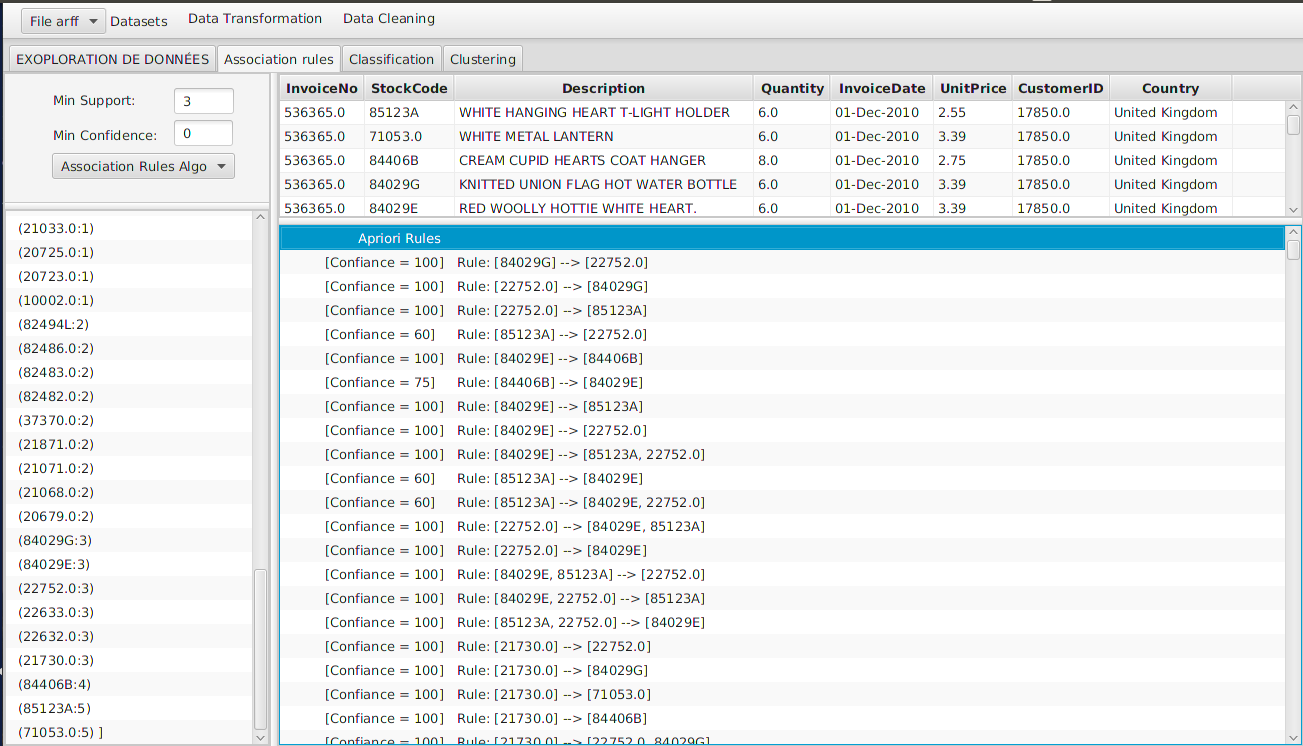
\includegraphics[width=1\textwidth]{images/apriori_supp3.png}%
			\captionof{figure}{Exécution d'Apriori avec Supp\_Min = 3}\label{labelname}%
		\end{minipage}
		\hspace{0.5cm}
		\begin{minipage}[b]{0.5\linewidth}
			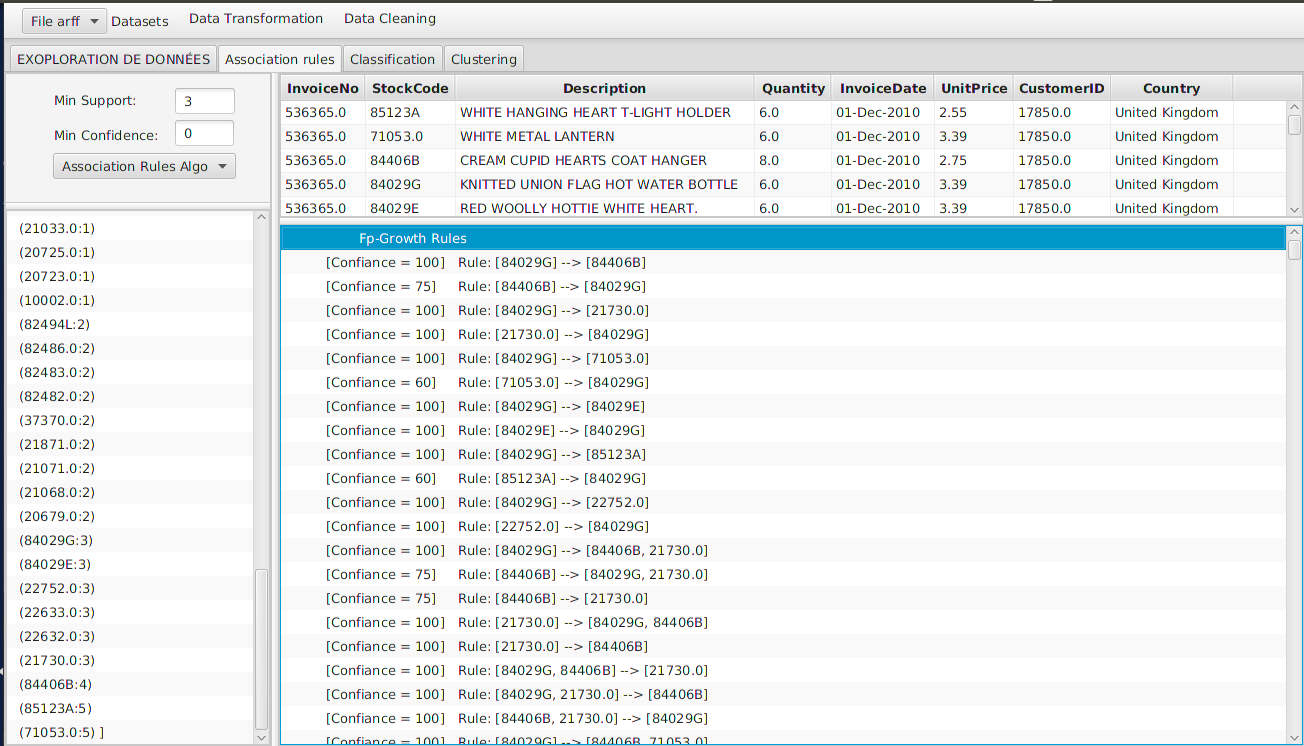
\includegraphics[width=1\textwidth]{images/fpg_supp3.png}%
			\captionof{figure}{Exécution de FP-Growth avec Supp\_Min = 3 }\label{labelname}%
		\end{minipage}
	\end{frame}
	
	\textbf{Remarque:}\\
	-Nous remarquons qu'avec les deux méthodes les mêmes règles sont générées, ce qui est tout à fait normal.\\
	-Nous avons généré une quantité importante de règles (plus de 100) avec des taux de confiance variant de \textbf{60\% à 100\%}.\\
	Chose que nous justifiant par le supprot minimal qui est assez petit, ainsi le nombre de régles est plus important, car il porte sur plus d'ItemSet (non éliminés).\\
	-Le temps d'exécution diffère entre les deux méthodes comme suit:
	\begin{center}
		\begin{tabular}{|p{5cm}|p{5cm}|}
			\hline
			\textbf{Apriori} &
			40 s
			\\
			\hline
			
			%\newline
			\textbf{FG-Growth} 
			%\newline
			&
			\textbf{ }%\newline
			5 s
			\\
			\hline
			
		\end{tabular} 
	\end{center}
	
	
	
	\subsubsection*{Configue 2 : Supp\_min : 4}
	
	\begin{frame}{}
		\centering
		\begin{minipage}[b]{0.5\linewidth}
			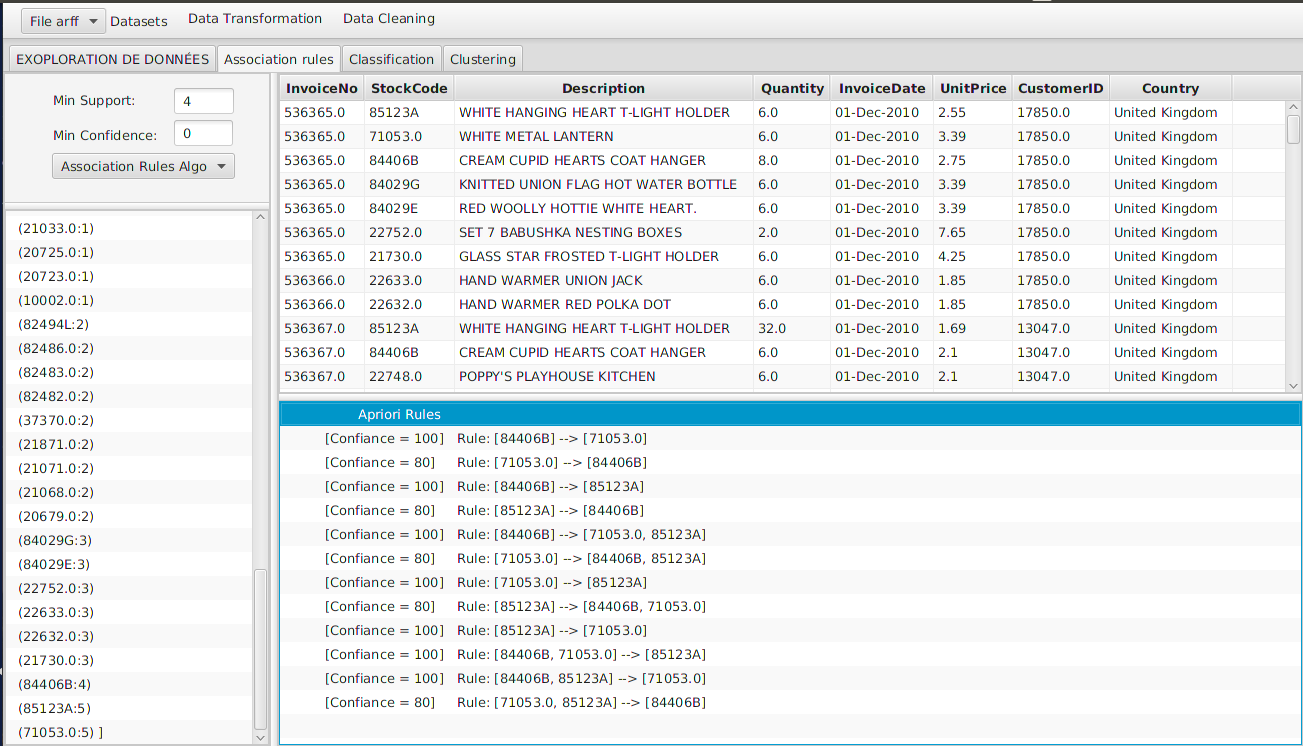
\includegraphics[width=1\textwidth]{images/apriori_supp4.png}%
			\captionof{figure}{Exécution d'Apriori avec Supp\_Min = 4}\label{labelname}%
		\end{minipage}
		\hspace{0.5cm}
		\begin{minipage}[b]{0.5\linewidth}
			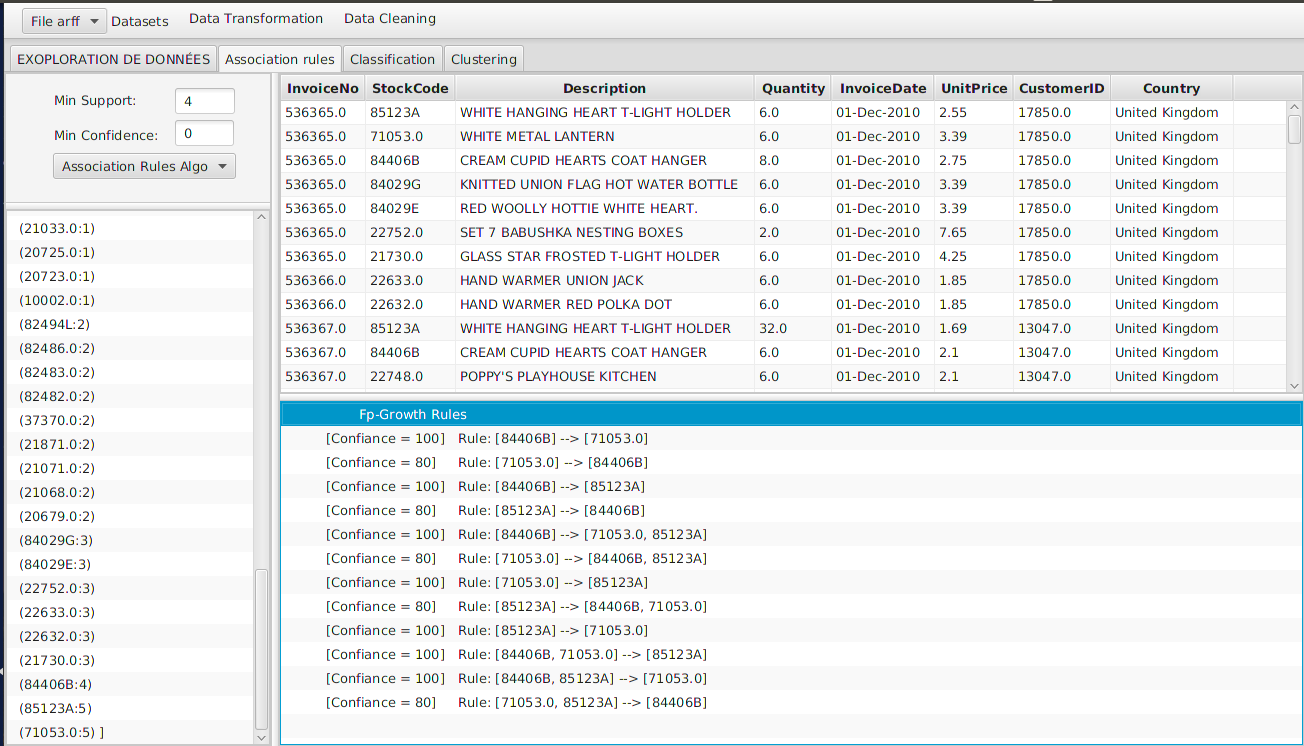
\includegraphics[width=1\textwidth]{images/fpg_supp4.png}%
			\captionof{figure}{Exécution de FP-Growth avec Supp\_Min = 4 }\label{labelname}%
		\end{minipage}
	\end{frame}
	
	\textbf{Remarque:}\\
	-Nous remarquons qu'avec les deux méthodes les mêmes règles sont générées encore une fois, ce qui est tout à fait normal.\\
	-Nous avons généré moins de règle (12 règles) comparé au nombre de règles générées avec un support minimal intérieur, et cela avec des taux de confiance de \textbf{80\% et 100\%}.\\
	Ainsi un support minimal plus élevé que le précédent a généré moins de règles, car il porte sur plus d'ItemSet ayant un support plus élevé, ce qui augmente le nombre d'ItemSet éliminés et donc réduit les possibilités.\\
	-Le temps d'exécution diffère entre les deux méthodes comme suit:
	\begin{center}
		\begin{tabular}{|p{5cm}|p{5cm}|}
			\hline
			\textbf{Apriori} &
			0.960 s
			\\
			\hline
			
			%\newline
			\textbf{FG-Growth} 
			%\newline
			&
			\textbf{ }%\newline
			0.601 s
			\\
			\hline
			
		\end{tabular} 
	\end{center}
	
	\subsubsection*{Configue 3 :Supp\_min : 5}
	
	\begin{frame}{}
		\centering
		\begin{minipage}[b]{0.5\linewidth}
			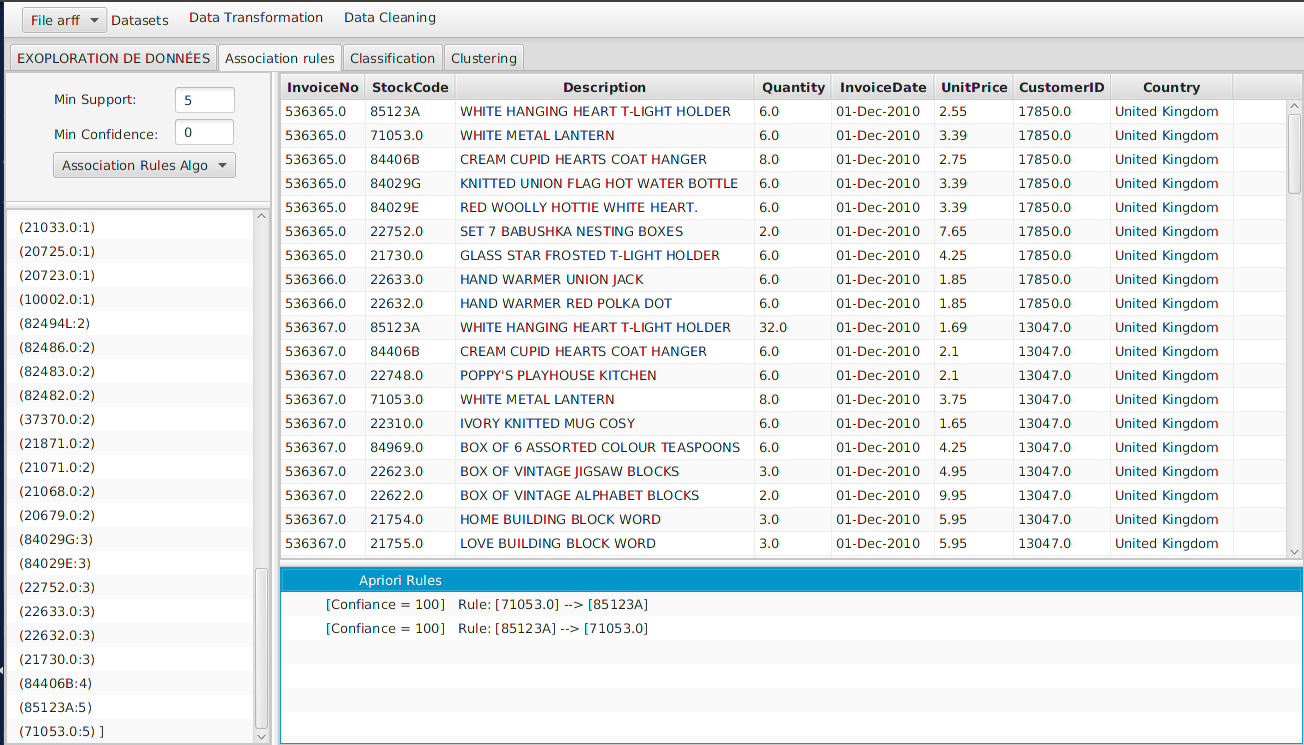
\includegraphics[width=1\textwidth]{images/apriori_supp5.png}%
			\captionof{figure}{Exécution d'Apriori avec Supp\_Min = 5}\label{labelname}%
		\end{minipage}
		\hspace{0.5cm}
		\begin{minipage}[b]{0.5\linewidth}
			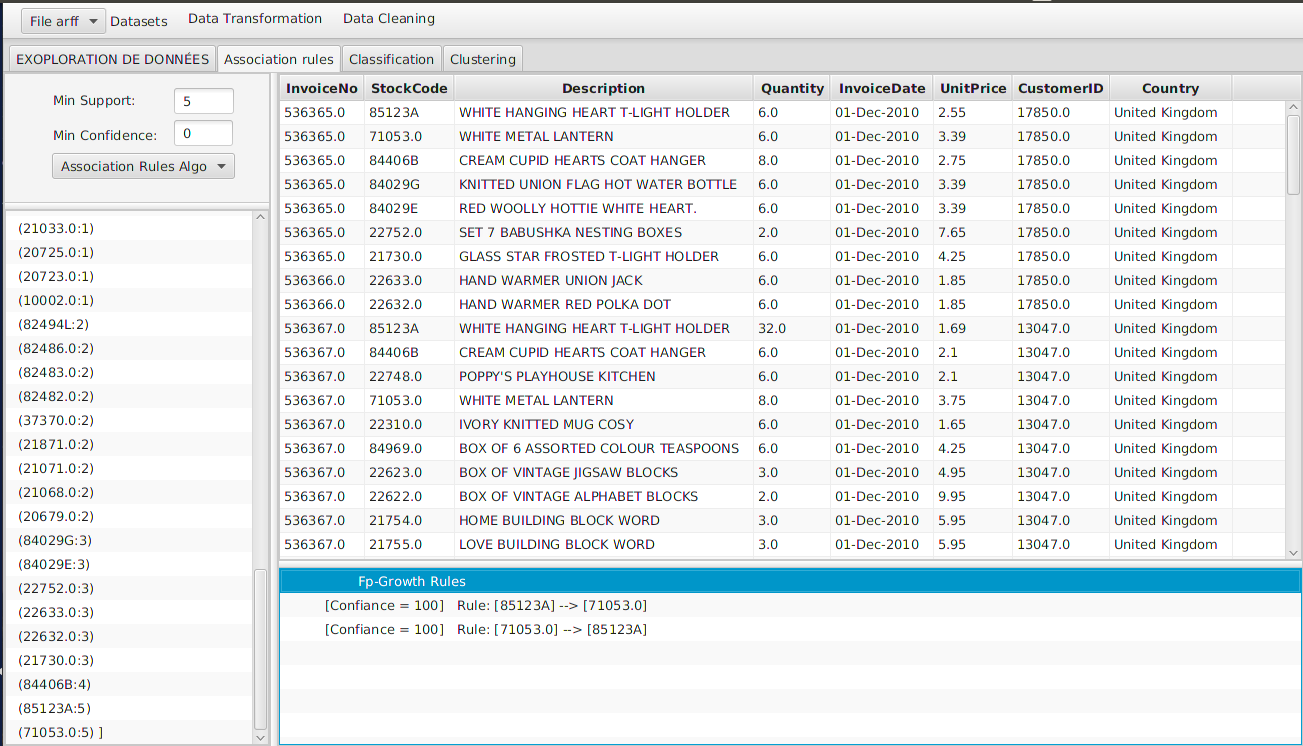
\includegraphics[width=1\textwidth]{images/fpg_supp5.png}%
			\captionof{figure}{Exécution de FP-Growth avec Supp\_Min = 5 }\label{labelname}%
		\end{minipage}
	\end{frame}
	
	
	\textbf{Remarque:}\\
	-Nous remarquons qu'avec les deux méthodes les mêmes règles sont générées encore une fois, ce qui est tout à fait normal.\\
	-Nous avons généré moins de règles (2 règles) comparé au nombre de règles générées avec un support minimal intérieur (3 et 4), et cela avec des taux de confiance de \textbf{ 100\%} pour les deux règles.\\
	Ainsi c'est le support minimal le plus élevé que l'on puisse utiliser pour obtenir des règles d'association car nous n'avons aucun Item ayant une fréquence supérieure à \textbf{5}.\\
	-Le temps d'exécution diffère entre les deux méthodes comme suit:
	
	
	\begin{center}
		\begin{tabular}{|p{5cm}|p{5cm}|}
			\hline
			\textbf{Apriori} &
			0.016 s
			\\
			\hline
			
			%\newline
			\textbf{FG-Growth} 
			%\newline
			&
			\textbf{ }%\newline
			0.006 s
			\\
			\hline
			
		\end{tabular} 
	\end{center}
	
	
	\vspace{2cm}
	\section{Conclusion}
	Pour finir ce chapitre, nous tenons à énumérer les points importants auxquels nous avons fait face lors de nos expérimentations sur Apriori et FP-Growth, c'est-à-dire:
	\begin{itemize}
		\item[$\bullet$] Plus le nombre de transaction est grand plus le temps d'exécution est important (élevé)
		\item[$\bullet$] Plus le Supp\_min est élevé moins les algorithmes ont d'itérations à faire, et donc plus le temps d'exécution est réduit.
		\item[$\bullet$] Les temps d'exécution de FP-Growth sont toujours plus faibles que ceux pour Apriori.\\
		
		Sauf lorsque le nombre d'itération est très petit, là nous avons pratiquement les mêmes temps d'exécution pour les deux approches.
		
		\begin{figure}[H]
			\centering
			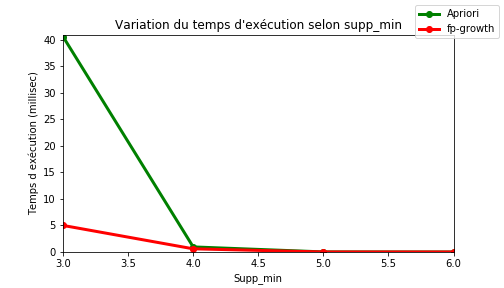
\includegraphics[scale=0.8]{image/ApFpPlot.png}
			\captionof{figure}{Variation du temps d'exécution selon supp\_min}\label{labelname}%
		\end{figure}
	\end{itemize}
	Aussi nous pouvons résumer notre étude comparative sur ces deux algorithme (Apriori et FP-Growth) en le tableau ci-dessous:
	
	\begin{center}
		\begin{tabular}{|p{5cm}|p{5cm}|p{5cm}|}
			\hline
			\textbf{Paramètre} &
			\textbf{Apriori} &
			\textbf{FG-Growth} 
			\\
			\hline
			
			%\newline
			Structure de stockage &
			Tableau (matrice) &
			Arbre 
			\\
			\hline
			
			%\newline
			Type de recherche &
			Largeur d'abord (toutes les combinaisons) &
			Diviser pour mieux régner + Profondeur d'abord
			\\
			\hline
			
			%\newline
			Techniques de bases &
			Génération de candidats, Jointure et filtrage &
			Extraire un sous arbre, Union et filtrage
			\\
			\hline	
			
			%\newline
			Nombre de scans du DataSet &
			K+1 scans &
			2 scans
			\\
			\hline	
			
			%\newline
			Espace mémoire &
			Grand &
			Petit
			\\
			\hline
			
			%\newline
			Temps d'exécution &
			Grand &
			Petit
			\\
			\hline		
			
			
		\end{tabular} 
	\end{center}
	
	En vu des résultats obtenus, on peut en conclure que l'algorithme FP-Growth est bien plus performant et intéressant à utiliser que l'algorithme Apriori.
	
	\chapter{Algorithme de classification : K-NN}
	\section{Introduction}
	%TODO han reference pour intro knn
	%blabla générale 3la les algo de classification (4 à 5 lignes hakak)
	K nearest neighbor où plutôt k plus proche voisins était décrit dans les \textbf{années 50} , c'est une méthode intensive qui demande beaucoup de temps de calcul pour arriver au résultat surtout quand il s'agit d'un large training sets, mais avec le développement des ordinateurs et la puissance de calcul son utilisation est revenu à l'actualité .[2]
	
	K NN fait partie des algorithmes de classification qui apprenne par analogie , donc il  se base sur des données d'entraînements (training set)
	pour prédire la classe des données de tests en faisant un calcul intensif de distance à chaque tuple des données de tests .
	
	\section{Principe de fonctionnement}
	On peut résumer le fonctionnement de l'algorithme K NN  dans les points suivants mais avant on doit définir quelques notions: 
	\subsection{Training set}
	un training set est un ensemble de données sur lequel s'opère l'analogie , ce choix est critique il doit être aussi diverse que possible pour couvrir toutes les possibilités dans le but de généraliser le  mieux par la suite , plus le training set est grand et divers plus la classification est susceptible d'être plus précise .
	\subsection{Testing set}
	le testing set est l'ensemble de données sur lequel on va tester notre modèle entraîné , il faut noter que les données du training et du set son de mème type , autrement dit ce sont des instances du même dataset.
	
	\subsection{Distance}
	K nn se base globalement sur le calcul de distance entre les instances du training set et celui du test set.
	
	Il existe pourtant plusieurs distances :
	\subsubsection{Distance Euclidienne}
	\begin{equation*}
	\begin{split}
	Distance(X_{1},X_{2}) =& \sqrt{ \sum_{i=1}^{n} (X_{1i} - X_{2i})^2}
	\end{split}
	\end{equation*}
	on l'utilise pour calculer la distance pour les attributs à valeurs numériques .
	\subsubsection{Distance Nominal}
	Pour la distance nominal on utilisé celle qui est "simple matching":
	\begin{equation}
	\begin{split}
	Distance(X_{1},X_{2}) =& \frac{p-m}{p}
	\end{split}
	\end{equation}
	
	où:
	
	\textbf{M}est le nombre d'attribut ou la valeur de l'instance $X_{1}$ est identique à celle de $X_{2}$ .
	
	\textbf{P} est le nombre total d'attribut ayant un type nominal .
	
	
	\subsubsection{Distance Hybride}
	Afin de calculer la distance entre deux instances ayant des attributs de type nominal et numérique on a utilisé la somme des deux distances nominal et numérique .
	\begin{equation*}
	\begin{split}
	Distance(X_{1},X_{2}) =& \sum \left \{ 
	\begin{array}{r c}
	X_{1} is numeric &  \sqrt{ \sum_{i=1}^{n} (X_{1i} - X_{2i})^2}\\
	X_{1} is nominal & \frac{P-M}{P}
	\end{array}
	\right .
	\end{split}
	\end{equation*}
	Plus la distance est grande moins les deux instances sont dites similaires et inversement .
	
	\subsection{Fonctionnement}
	
	Ainsi on peut résumer le principe  de fonctionnement comme suit:
	\begin{enumerate}
		\item Partitionner les données en ensemble de test et training
		\item Pour chaque instance de l'ensemble de test faire 
		\item Calculer la distance entre l'instance courante du test et toutes les instances du training set les mettre avec la classe correspondante , au fur et à mesure dans un tableau ou une liste.
		\item Trier le tableau de distance par ordre croissant 
		\item prendre Les K premiers éléments de la liste  et calculer le mode ( la classe la plus fréquente)
		\item Attribuer la classe trouvée en calculant le mode à l'instance du test set courante .
	\end{enumerate}
		\textbf{Complexité:}\\
		
		La complexité Temporelle de \textbf{Knn} est Polynomial quadratique,  en \textbf{\textit{O($taille(trainingset)^2*taille(testset)$)}}.
		
		car on fait un tri sur un tableau comportant les distances de l'instance du test set à classifier  avec tout le Training-set, la fonction de tri étant de complexité quadratique.
		
		La complexité Spatial  de \textbf{Knn} est en \textbf{\textit{O(n)}}.
		
		
		Avec: $n$ : nombre d'instances du DataSet (test + training).
	
	\section{Structures de données}
	Dans le but d'implémenter notre algorithme de classification  K NN on a opté pour la modélisation suivante:
	
	\subsection{Element}
	
	\begin{itemize}
		\item   \textbf{  Classi}: qui est la classe de l'élément
		\item \textbf{distance:} qui est la distance associé à l'élément de type réel (float ou double)
		
	\end{itemize}
	\subsection{VecteurD(Vecteur de distances)}
	
	\begin{itemize}
		\item\textbf{ ListofDistances:} qui est une liste contenant des ELEMENT( décrit plus haut) 
	\end{itemize}
	la liste de distance étant nécessaire pour notre modélisation a fin de faire un tri décroissant sur cette liste selon la distance  et récupérer ainsi les K PREMIÈRES Distances associées au instances puis ainsi on pourra extraire le mode dans ces K premières distances. 
	\section{Pseudo-code}
	
	\begin{algorithm}[H]
		\DontPrintSemicolon
		\KwIn{TrainingSet : dataset qui sert à faire l'apprentissage,\\
			\hspace{1.45cm}TestSet : Données à classer,\\
			\hspace{1.5cm}K : nombre de voisins}
		\KwOut{TestSetClassé : les données classifiées	}
		
		
		\For{$instance1  \in TestingSet $}{	
			
			\For{$instance2  \in TrainingSet $}
			{	
				List\_distance.add(CalculDistance(instance1,instance2))
				
			}
			List\_distance $\gets$ Trier(List\_distance)
			
			Class $\gets$ K-MostcommonClass(List\_distance,K)\\
			$Instance1.Class \gets Class$\\
			TestSetClassé.add($Instance1$)
		}	  
		
		\Return{$TestSetClasse$}\;
		\caption{{\sc K NN:()}}
		\label{algo:duplicate1}
	\end{algorithm}

	
	\section{Résultats}
	Pour la méthode de classification supervisé KNN les paramètres empiriques sont le K et la taille du training et test set .
	on a donc fait varier K et  la taille des trainingset et testset et voir comment ils influencent la précision.
	
	Pour la précision on l'a calculé comme suit : 
	\begin{equation*}
	Accuracy=\frac{VraiPositives}{Taille(Testset)}
	\end{equation*}
	on a aussi décidé d'étudier les variations du temps d'exécution en fonction de nos paramètres  les résultats sont les suivants :
	\subsection{Dataset: labor }
	
	\subsubsection{Trainingset:90 et TestSET:10}
	\textbf{Temps d'exécution + précision}\\
	\begin{frame}{}
		\centering
		\begin{minipage}[b]{0.5\linewidth}
			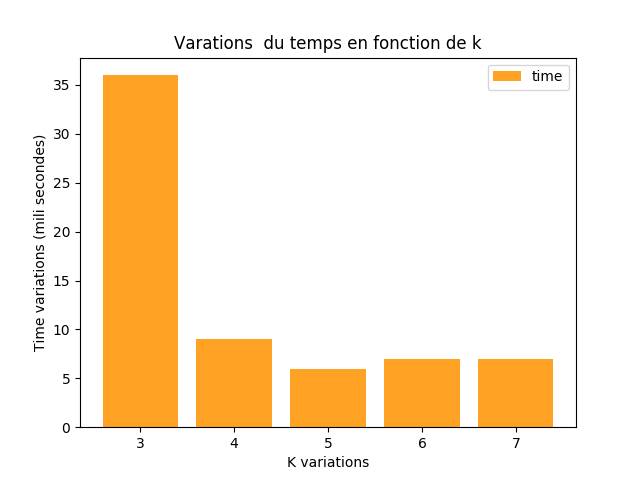
\includegraphics[scale=0.5]{image/labor:Train,90,Test,10time.png}
			\captionof{figure}{Variations du temps en fonction de K}\label{labelname}%
		\end{minipage}
		\hspace{0.5cm}
		\begin{minipage}[b]{0.5\linewidth}
			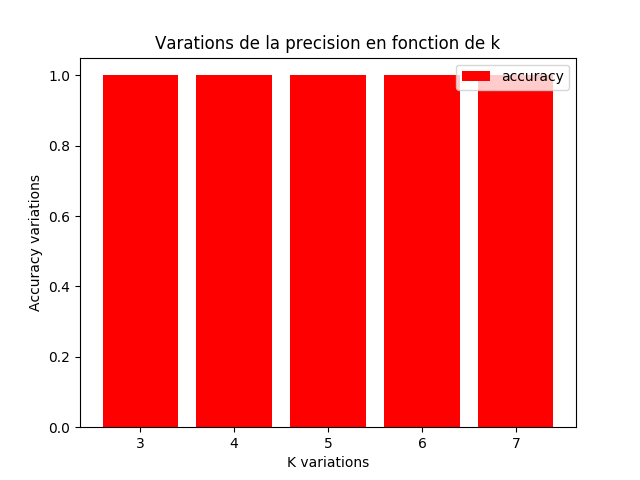
\includegraphics[scale=0.5]{image/labor:Train,80,Test,20:accuracy.png}%
			\captionof{figure}{Variations de la précision en fonction de K }\label{labelname}%
		\end{minipage}
	\end{frame}
	
	
	
	
	\subsubsection{Trainingset:80 et TestSET:20}
	
	\textbf{Temps d'exécution + précision}\\
	\begin{frame}{}
		\centering
		\begin{minipage}[b]{0.5\linewidth}
			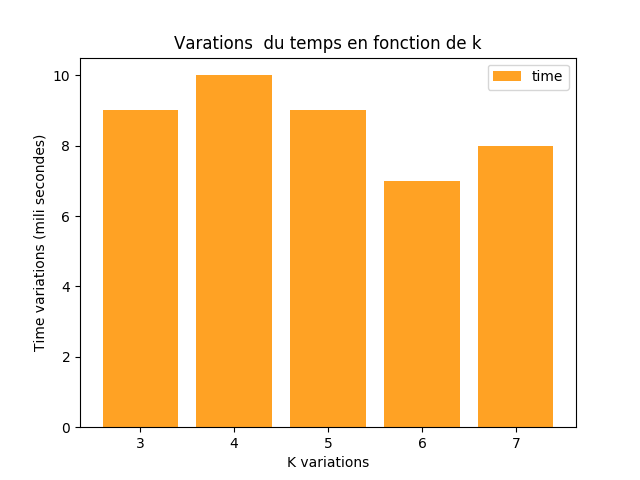
\includegraphics[scale=0.5]{image/labor:Train,80,Test,20time.png}
			\captionof{figure}{Variations du temps en fonction de K}\label{labelname}%
		\end{minipage}
		\hspace{0.5cm}
		\begin{minipage}[b]{0.5\linewidth}
			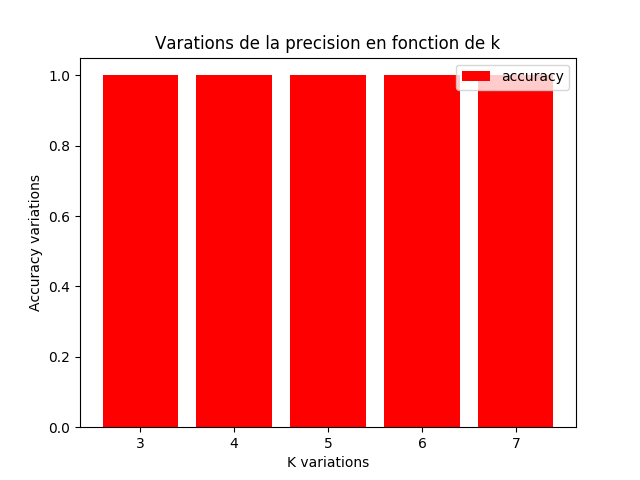
\includegraphics[scale=0.5]{image/labor:Train,80,Test,20:accuracy.png}%
			\captionof{figure}{Variations de la précision en fonction de K }\label{labelname}%
		\end{minipage}
	\end{frame}
	
	
	
	\subsubsection{Trainingset:70 et TestSET:30}
	\textbf{Temps d'exécution + précision}\\
	\begin{frame}{}
		\centering
		\begin{minipage}[b]{0.5\linewidth}
			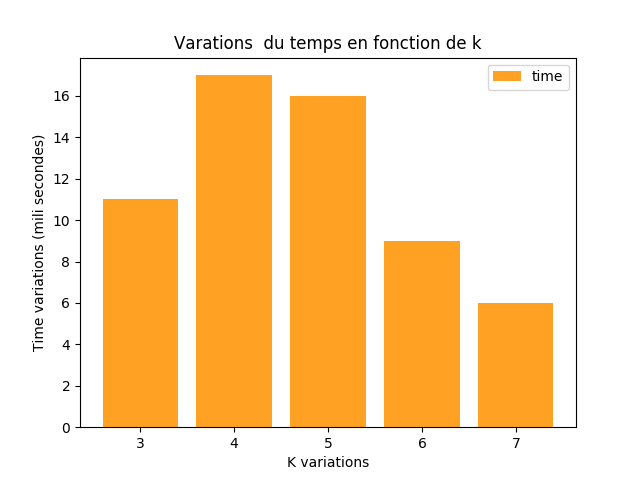
\includegraphics[scale=0.5]{image/labor:Train,70,Test,30time.png}
			\captionof{figure}{Variations du temps en fonction de K}\label{labelname}%
		\end{minipage}
		\hspace{0.5cm}
		\begin{minipage}[b]{0.5\linewidth}
			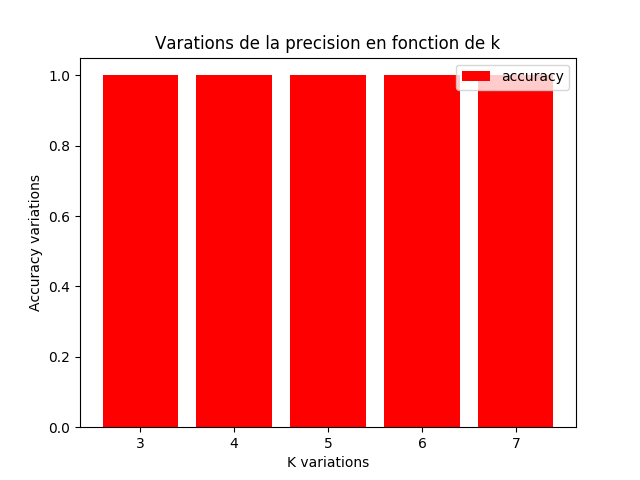
\includegraphics[scale=0.5]{image/labor:Train,70,Test,30:accuracy.png}%
			\captionof{figure}{Variations de la précision en fonction de K }\label{labelname}%
		\end{minipage}
	\end{frame}
	
	
	
	
	\subsubsection{Trainingset:60 et TestSET:40}
	\textbf{Temps d'exécution + précision}\\
	\begin{frame}{}
		\centering
		\begin{minipage}[b]{0.5\linewidth}
			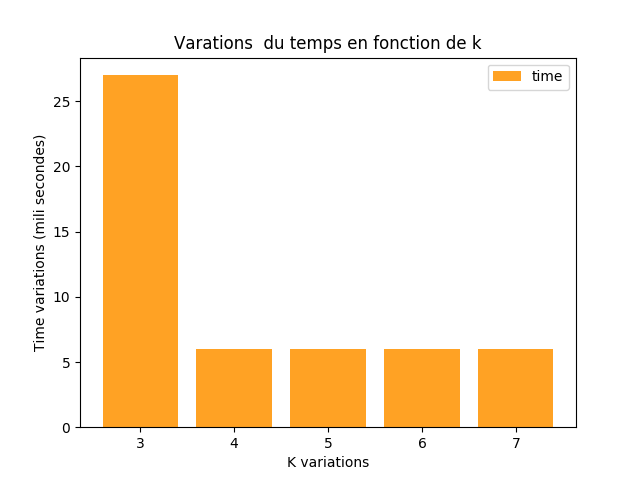
\includegraphics[scale=0.5]{image/labor:Train,60,Test,40time.png}
			\captionof{figure}{Variations du temps en fonction de K}\label{labelname}%
		\end{minipage}
		\hspace{0.5cm}
		\begin{minipage}[b]{0.5\linewidth}
			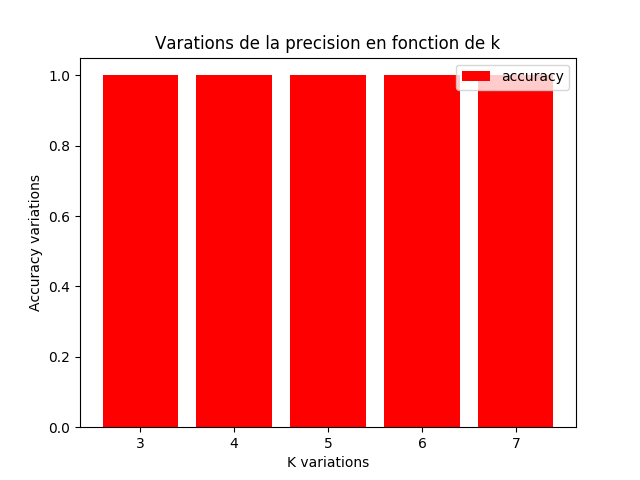
\includegraphics[scale=0.5]{image/labor:Train,60,Test,40:accuracy.png}%
			\captionof{figure}{Variations de la précision en fonction de K }\label{labelname}%
		\end{minipage}
	\end{frame}
	
	
	\subsubsection{Trainingset:50 et TestSET:50}
	
	\textbf{Temps d'exécution + précision}\\
	\begin{frame}{}
		\centering
		\begin{minipage}[b]{0.5\linewidth}
			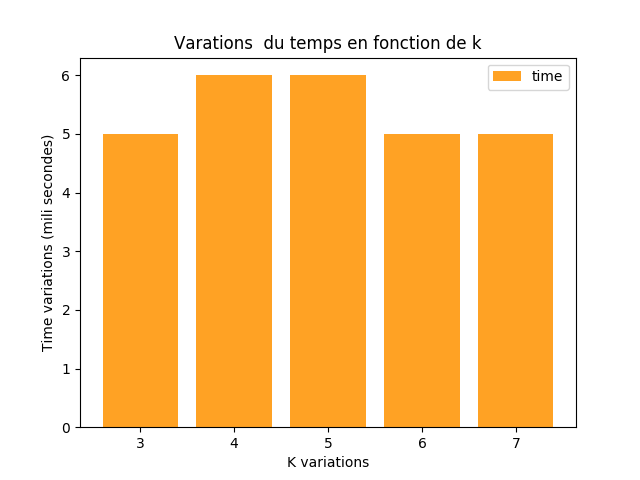
\includegraphics[scale=0.5]{image/labor:Train,50,Test,50time.png}
			\captionof{figure}{Variations du temps en fonction de K}\label{labelname}%
		\end{minipage}
		\hspace{0.5cm}
		\begin{minipage}[b]{0.5\linewidth}
			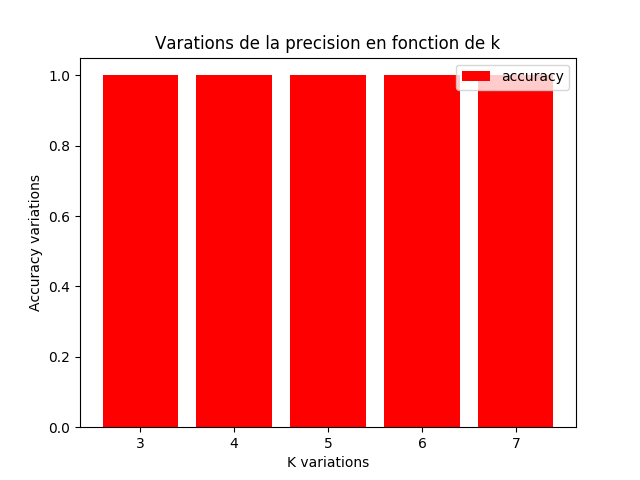
\includegraphics[scale=0.5]{image/labor:Train,50,Test,50:accuracy.png}%
			\captionof{figure}{Variations de la précision en fonction de K }\label{labelname}%
		\end{minipage}
	\end{frame}
	
	

	
	
	
	\subsection{Dataset: Unbalanced (numérique)}
	unbalanced est un data set numerique avec une classe binaire (active ,non active) il comporte plus de 800 instanes et 37 attributs .
	
	\subsubsection{Trainingset:90 et TestSET:10}
	\textbf{Temps d'exécution + précision}\\
	\begin{frame}{}
		\centering
		\begin{minipage}[b]{0.5\linewidth}
			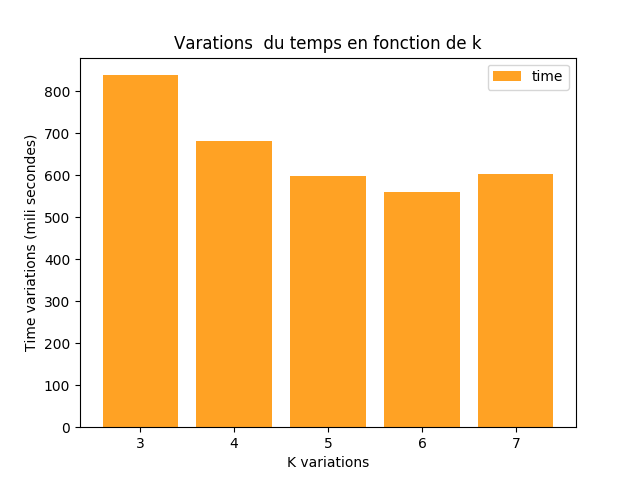
\includegraphics[scale=0.5]{image/data2:Train,90,Test,10time.png}
			\captionof{figure}{Variations du temps en fonction de K}\label{labelname}%
		\end{minipage}
		\hspace{0.5cm}
		\begin{minipage}[b]{0.5\linewidth}
			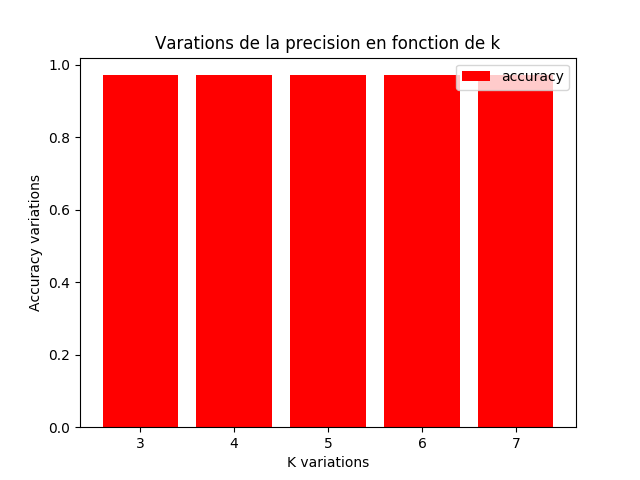
\includegraphics[scale=0.5]{image/data2:Train,80,Test,20:accuracy.png}%
			\captionof{figure}{Variations de la précision en fonction de K }\label{labelname}%
		\end{minipage}
	\end{frame}
	
	
	\subsubsection{Trainingset:80 et TestSET:20}
	\textbf{Temps d'exécution + précision}\\
	\begin{frame}{}
		\centering
		\begin{minipage}[b]{0.5\linewidth}
			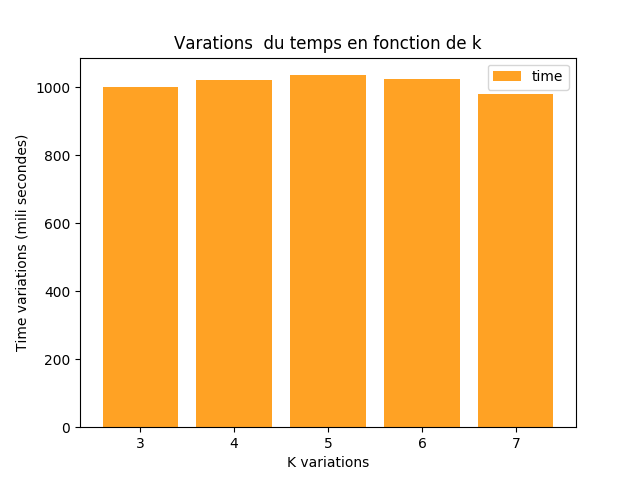
\includegraphics[scale=0.5]{image/data2:Train,80,Test,20time.png}
			\captionof{figure}{Variations du temps en fonction de K}\label{labelname}%
		\end{minipage}
		\hspace{0.5cm}
		\begin{minipage}[b]{0.5\linewidth}
			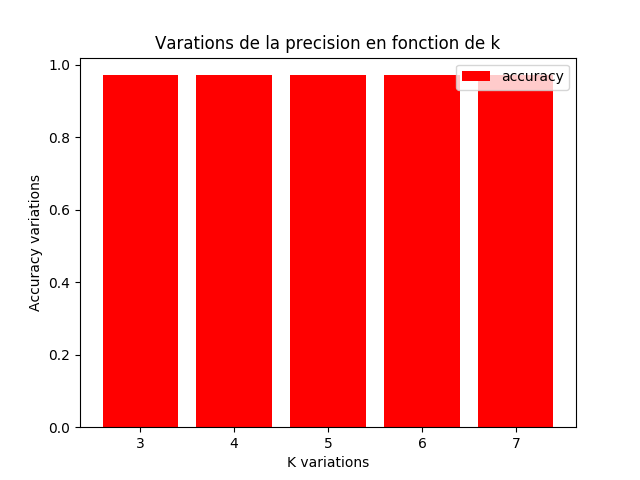
\includegraphics[scale=0.5]{image/data2:Train,80,Test,20:accuracy.png}%
			\captionof{figure}{Variations de la précision en fonction de K }\label{labelname}%
		\end{minipage}
	\end{frame}
	
	
	\subsubsection{Trainingset:70 et TestSET:30}
	\textbf{Temps d'exécution + précision}\\
	\begin{frame}{}
		\centering
		\begin{minipage}[b]{0.5\linewidth}
			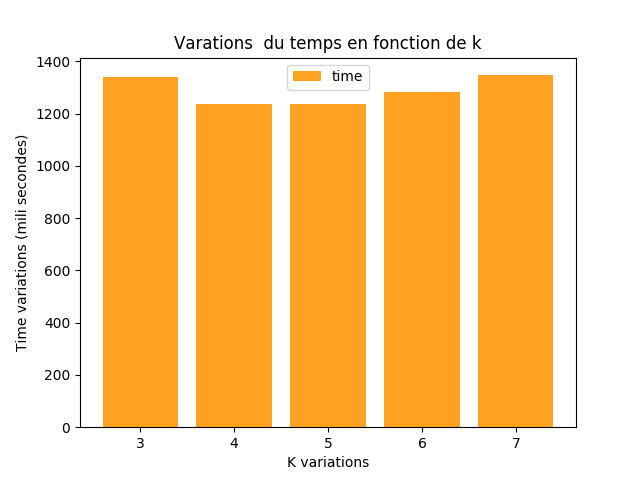
\includegraphics[scale=0.5]{image/data2:Train,70,Test,30time.png}
			\captionof{figure}{Variations du temps en fonction de K}\label{labelname}%
		\end{minipage}
		\hspace{0.5cm}
		\begin{minipage}[b]{0.5\linewidth}
			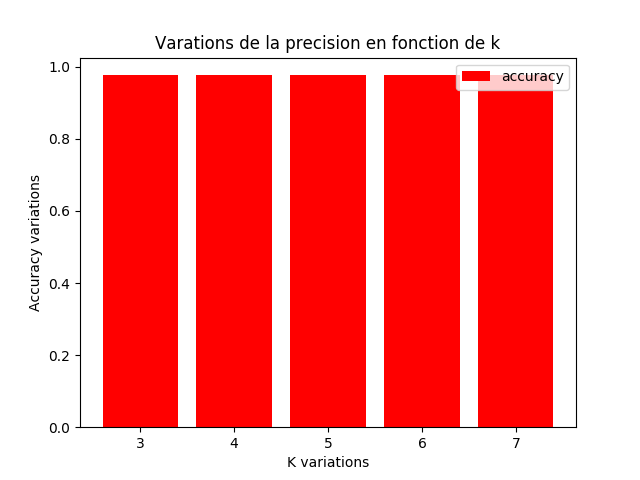
\includegraphics[scale=0.5]{image/data2:Train,70,Test,30:accuracy.png}%
			\captionof{figure}{Variations de la précision en fonction de K }\label{labelname}%
		\end{minipage}
	\end{frame}
	
	
	\subsubsection{Trainingset:60 et TestSET:40}
	\textbf{Temps d'exécution + précision}\\
	\begin{frame}{}
		\centering
		\begin{minipage}[b]{0.5\linewidth}
			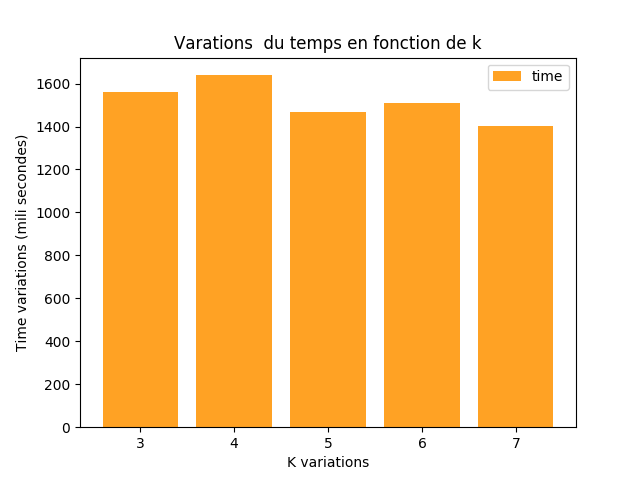
\includegraphics[scale=0.5]{image/data2:Train,60,Test,40time.png}
			\captionof{figure}{Variations du temps en fonction de K}\label{labelname}%
		\end{minipage}
		\hspace{0.5cm}
		\begin{minipage}[b]{0.5\linewidth}
			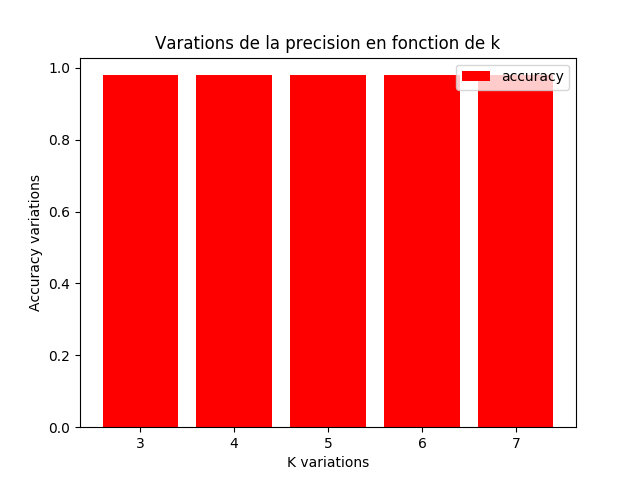
\includegraphics[scale=0.5]{image/data2:Train,60,Test,40:accuracy.png}%
			\captionof{figure}{Variations de la précision en fonction de K }\label{labelname}%
		\end{minipage}
	\end{frame}
	
	
	\subsubsection{Trainingset:50 et TestSET:50}
	\textbf{Temps d'exécution + précision}\\
	\begin{frame}{}
		\centering
		\begin{minipage}[b]{0.5\linewidth}
			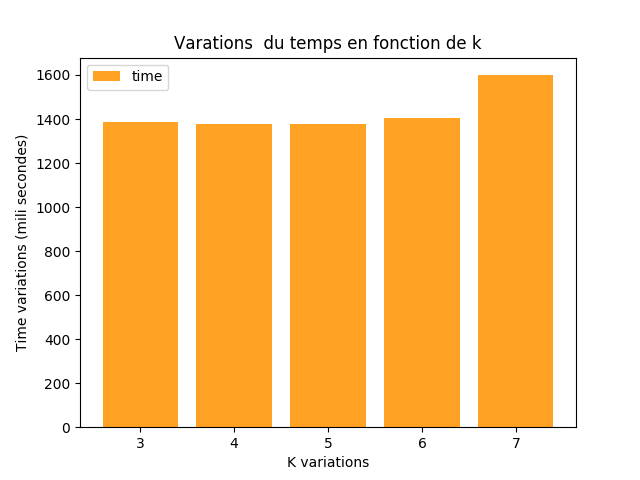
\includegraphics[scale=0.5]{image/data2:Train,50,Test,50time.png}
			\captionof{figure}{Variations du temps en fonction de K}\label{labelname}%
		\end{minipage}
		\hspace{0.5cm}
		\begin{minipage}[b]{0.5\linewidth}
			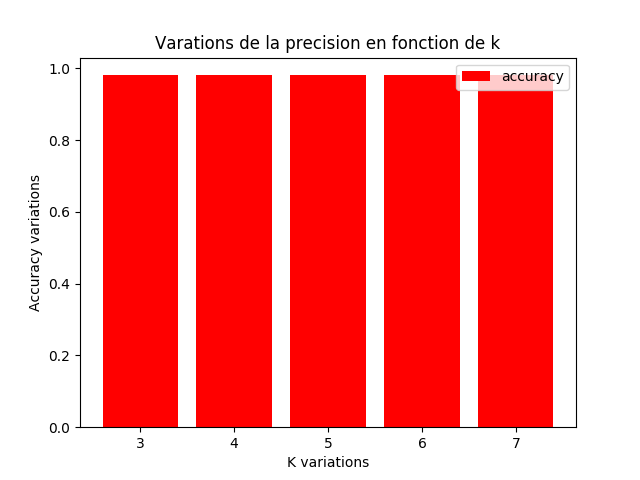
\includegraphics[scale=0.5]{image/data2:Train,50,Test,50:accuracy.png}%
			\captionof{figure}{Variations de la précision en fonction de K }\label{labelname}%
		\end{minipage}
	\end{frame}
	
	\subsubsection{Trainingset:80 et test:20 avec K=7,13,20}
	
	 on a pri
		\textbf{Temps d'exécution + précision}\\
		\begin{frame}{}
			\centering
			\begin{minipage}[b]{0.5\linewidth}
				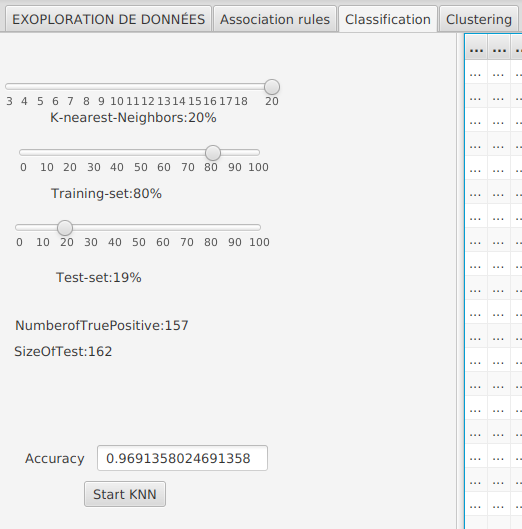
\includegraphics[scale=0.5]{image/k=20unbalanced.png}
				\captionof{figure}{Précision pour K=20 pour dataset unbalanced}\label{labelname}%
			\end{minipage}
			\hspace{0.25cm}
			\begin{minipage}[b]{0.5\linewidth}
				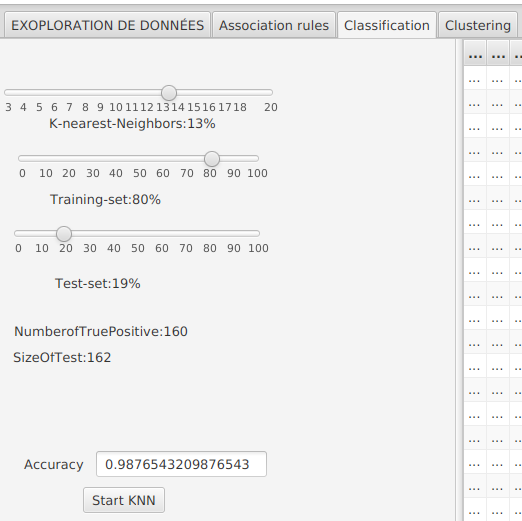
\includegraphics[scale=0.5]{image/k=13unbalanced.png}%
				\captionof{figure}{Précision pour k=13 pour dataset unbalanced }\label{labelname}%
			\end{minipage}
		\end{frame}
		
	\begin{minipage}[b]{0.5\linewidth}
		\centering
		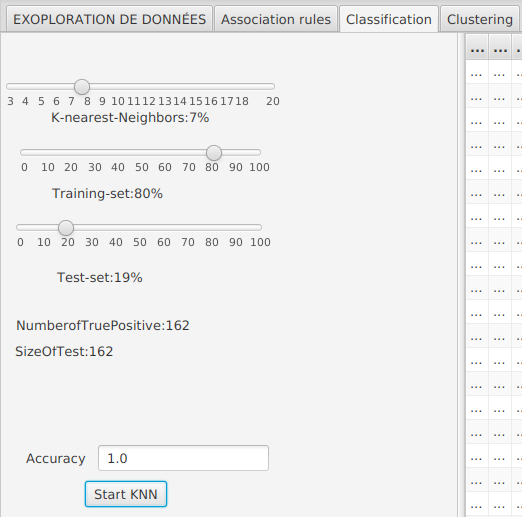
\includegraphics[scale=0.5]{image/k=7unbalanced.png}%
		\captionof{figure}{Précision pour k=7 pour dataset unbalanced }\label{labelname}%
	\end{minipage}
	\paragraph{Remarques}
	On remarque clairement que pour le dataset unbalanced après normalisation et nettoyage on a eu :
	\begin{center}
		\begin{tabular}{ | l || c | c | c | }
			\hline
		\textbf{K} & 7 & 13 & 20\\
		 \hline
			\textbf{ Précision} & 100\%  & 98\%  & 96\% \\
			\hline
		\end{tabular}
	\end{center}
	
	K et la précision sont inversement proportionnelle c'est à dire si K augmente on peut noter que la précision diminue cela peut être expliqué par la confusion  que rencontre KNN lorsque le nombre de plus proche voisins à considérer est important , la classe modale varie et on va prendre des voisins qui sont de plus en plus loin de notre instance à classifier.
	
	
	
	\newpage
	
	\section{Conclusion}
	Selon nos expérimentations on a pu remarquer les points suivants :
	%TO DO: ajouter un test avec k 20 sur l'interface lol
	
	
	\begin{itemize}
		\item L'approche K-nn est caractérisé par le paramètre \textbf{K} qui est le nombre de voisin à prendre en compte pour classer une instance, ce paramètre doit être fixé suite à plusieurs expérimentations.
		
		\item Les variations de K  (de 3 jusqu'à 7 ) n'influencent  pas énormément la précision par contre elle augmente parfois le temps d'exécution. mais si on augmente K à des valeurs conséquentes par exemple 20 etc , on remarque que la précision diminue car on s'intéresse plus aux classes des premières instances vu qu'on va prendre 20 voisins et la classe modale  par rapport à ces voisins (20), une solution serait de pondérés les K élément en donnant un poids à chaque instance trouvée dans les K voisins en mettant en priorité celles qui sont proches (un peu comme dans la recherche d'information).
		
		\item les variations du training set et test set ont influencé la précision on remarque que plus on augmente le testset et on diminue le training set plus la précision diminue, ceci peut être expliqué par le fait que  le training set ne devient plus assez diverse (il est même possible qu'une classe entière ne soit pas représenté), donc les données de test deviennent inconnues et il ne saura pas comment les classifier.
		\item On a noté aussi que KNN est trés sensible au bruit et à la normalisation , par exemple on a eu des précisions de 45\% pour le dataset labor SANS normalisation et sans nettoyage alors que aprés le prétraitement on eu prés de 98\% ceci est en relation direct avec le calcul de distance , un attribut dominera la classification ( il convergera cette dernière)  si il a des valeurs assez grandes et inversement un attribut aura moins d'effet si ces valeurs sont petites on parle ici du cas numérique.
	\end{itemize}
	\chapter{Algorithme de clustering : DBSCAN}
	\section{Introduction}
	Le Clustering consiste en un regroupement d'objets (instances) dans un même cluster/groupe selon la similitude qui les rassemble, c'est à dire en comparant les caractéristiques de ces objets (instances) nous obtenons une distance que l'on cherche à minimiser entre deux objets du même cluster et à maximiser entre deux clusters.\\
	
	Parmi les méthodes de clustering nous avons quatre catégories: 
	\begin{itemize}
		\item[$\bullet$] Méthodes basées Partitionnement
		\item[$\bullet$] Méthodes Hiérarchiques
		\item[$\bullet$] Méthodes basées Densité
		\item[$\bullet$] Méthodes basées Grille
	\end{itemize}
	
	\section{Principe de fonctionnement}
	\textbf{DBSCAN} a été proposé en \textbf{1996} par Martin.E et al. Il est basé sur la densité, Il procède à la création des clusters de manière incrémentale c'est-à-dire qu'il crée et fini de remplir un cluster avant de passer au suivant, ainsi cet algorithme prend deux paramètres empiriques qui sont:
	\begin{itemize}
		\item[$\bullet$] \textbf{epsilon ($\epsilon$) :} la distance maximale entre deux objets (instances) pour qu'ils soient considérés comme voisins.
		\item[$\bullet$] \textbf{MinPts :} Le nombre minimum de voisins pour créer un cluster.
	\end{itemize}
	
	\textbf{ }\\
	\textbf{Complexité:}\\
	La complexité Temporelle de \textbf{dbscan} est Polynomial,  en \textbf{\textit{O($n^2$)}}.\\
	La complexité Spatiale  de \textbf{dbscan} est en \textbf{\textit{O(n)}}.
	
	
	Avec: $n$ : nombre d'instances du DataSet.
	
	
	
	
	\section{Structures de données}
	\subsection*{Cluster}
	Nous avons défini la structure de \textbf{Cluster}, celle-ci représente un Cluster contenant l'ensemble des instances qu'il regroupe, telle qu'elle est composée de 2 attributs:
	\begin{itemize}
		\item[$\bullet$] \textbf{clusterName:}chaine de caractère représentant le nom du Cluster. (\textit{exemple: "cluster1"})
		\item[$\bullet$] \textbf{listInstances:} La liste des instances appartenant a ce Cluster.
	\end{itemize}
	
	\subsection*{dbscan}
	Il s'agit d'une instance pour l'exécution de dbscan, telle que les éléments de base nécessaires pour cela y sont structuré comme suit:
	\begin{itemize}
		\item[$\bullet$] \textbf{DataSet:} le dataset contenant les instances que nous souhaitons clusteriser.
		\item[$\bullet$] \textbf{epsilon ($\epsilon$):} distance maximal pour considérer une instance comme un voisin d'une autre instance.
		\item[$\bullet$] \textbf{MinPts:} le nombre minimal de voisins pour un point afin de le regrouper dans un cluster.
		
	\end{itemize}
	
	
	
	
	\section{Pseudo-code}
	
	\begin{algorithm}[H]
		\DontPrintSemicolon
		\KwIn{D:Dataset à clusteriser ,$Epsilon (\epsilon)$ :distance minimal d'un voisin,
			$MinPts$ : nombre minimum de voisins}
		\KwOut{$Clusters$: Liste des clusters}
		
		\textbf{ }\\
		\ForEach{Point P $\in$ D}{
			MarquéVisité(P)\\
			$PtsVoisins \gets $ Voisinage(D,P,epsilon)\\
			
			\If{Taille($PtsVoisins$) $<$ $MinPts$}{
				$BruitList$.add(P)\;\\
				//marquer P comme du bruit
			}\Else{
			$NewCluster \gets$ CreationCluster()\;\\ EtendreCluster(D, P, PtsVoisins, NewCluster, epsilon, MinPts)\;\\
			$Clusters.add$($NewCluster$)
		}
	} 
	
	
	\Return{$Clusters$}\;
	\caption{\sc DBSCAN}
\end{algorithm}


\begin{algorithm}[H]
	\SetAlgoLined
	\DontPrintSemicolon
	\textbf{EtendreCluster(D, P, PtsVoisins, NewCluster, epsilon, MinPts)}\;
	
	$NewCluster \gets$ Inserer(P)\\
	\ForEach{$Point P' \in PtsVoisins$}{
		\If{$P'$ nonVisité}{
			MarquéVisité($P'$)\\
			$PtsVoisins' \gets$ Voisinage(D,$P'$,epsilon)\\
			\If{Taille($PtsVoisins'$) $\geq$ $MinPts$}{
				$PtsVoisins = PtsVoisins \cup PtsVoisins'$
			}
		}
		\If{$P' \notin Any Cluster$}{  
			$NewCluster \gets $Inserer(P') 
		}
	}
	
	\caption{\sc Procedure EtendreCluster}
\end{algorithm}

\begin{algorithm}[H]
	\SetAlgoLined
	\DontPrintSemicolon
	\textbf{Voisinage(D, P, epsilon)}\;
	
	\ForEach{$Points Pts \in D$}{
		\If{Distance(P,Pts) $\leq$ epsilon}{
			$listVoisins$.add(Pts)
		}
	}
	
	\Return{$listVoisins$}
	\caption{\sc Voisinage}
	
\end{algorithm}


\section{Explication}
\begin{enumerate}
	
	
	\item Sélectionner aléatoirement un point \textbf{p}, le marqué comme \textit{"visité"} c'est-à-dire clusterisé.
	
	\item Récupérer tous les points accessibles en densité à partir de \textbf{p}, c'est-à-dire distance entre \textbf{p} et ces autres points $\leq$ Epsilon ($\epsilon$), on appelle ces points les voisins de \textbf{p}.
	
	\item Si le nombre de voisins de \textbf{p} est $\geq$ MinPts,Alors \textbf{p} est un \textbf{corps}, on forme un nouveau cluster.\\
	
	Puis on procède de la même manière pour ces voisins de \textbf{p}, mais cette fois on ne crée pas un nouveau cluster mais on les ajoute au cluster de \textbf{p}.
	
	\item Sinon \textbf{p} est un point frontière, c'est-à-dire aucun point n'est accessible en densité à partir de \textbf{p}.
	
	\item DBSCAN visite le prochain point du Dataset non clusterisé.
	
	\item Si un point ne peux être ajouté dans aucun cluster et ne peux pas être un point corps pour un nouveau cluster (epsilon,MinPts non compatible) alors marquer le point comme bruit.
	
	\item Continuez le processus jusqu'à ce que tous les points aient été traités.
\end{enumerate}


\subsubsection*{Évaluation:}
Il existe des mesures d'évaluation du clustering obtenu, nous citons: \textbf{L'Inertie Inter-Cluster} et \textbf{Intra-Cluster}, tel que:
\begin{itemize}
	\item \textbf{Intra-Cluster :} elle représente la somme des inerties de tous les clusters 
	La formule d'évaluation est comme suit:
	\begin{center}
		$\sum_{i=1}^{nbrCluster} \sum_{X_i \in C_i} d^{2}(X_i , G_i) $
	\end{center}
	Avec:\\
	$C_i$ : $i^{eme}$ cluster.\\
	$G_i$ : Centre de gravité du $i^{eme}$ cluster.\\
	$X_i$ : Instance du $i^{eme}$ cluster.\\
	$d$ : distance euclidienne.\\
	
	
	\item \textbf{Inter-Cluster :} cette mesure permet de mesurer la disparité des clusters, c'est à dire la distance entre clusters, celle-ci doit être élevée pour rester cohérent dans la logique du clustering.\\
	La formule d'évaluation est la suivante:
	\begin{center}
		$\sum_{i=1}^{nbrCluster} d^{2}(G_i , Gl) $
	\end{center} 
	Avec:\\
	$G_i$ : Centre de gravité du $i^{eme}$ cluster.\\
	$Gl$ : Centre de gravité globale (de tous le nuage de points).\\
	$d$ : distance euclidienne.
	
\end{itemize} 

\subsubsection*{Remarque 1:}
Il existe la version normalisée de ces mesures, qui sont comme suit:\\

Intra : 
$ \langle\sum_{i=1}^{nbrCluster} \sum_{X_i \in C_i} d^{2}(X_i , G_i) \rangle / nbrInstancesClusterisees$

\vspace{0.5cm}
Inter : 
$\langle\sum_{i=1}^{nbrCluster} d^{2}(G_i , Gl) \rangle /  nbrCluster$

\subsubsection*{Remarque 2:}
Ces deux mesures sont mises en comparaison, pour dire que nous avons un bon clustering, il faut que 2 points soient visibles :

$\bullet$ Nos Clusters soient danses $\Leftrightarrow$ minimiser la mesure intra-Cluster.


$\bullet$ Nos Clusters soient éloignés (clairement disjoint) $\Leftrightarrow$ maximiser la mesure inter-Cluster.
\newpage

\section{Résultats}
\subsubsection*{DataSet : LABOR (57 instance/17 attributs)}

\begin{itemize}
	\item[$\bullet$] \textbf{Mixte (Nominal + numérique)}
	\item[$\bullet$] \textbf{Epsilon = 1.7}
	\item[$\bullet$] \textbf{MinPts = 3}
\end{itemize}

\begin{figure}[H]
	\centering
	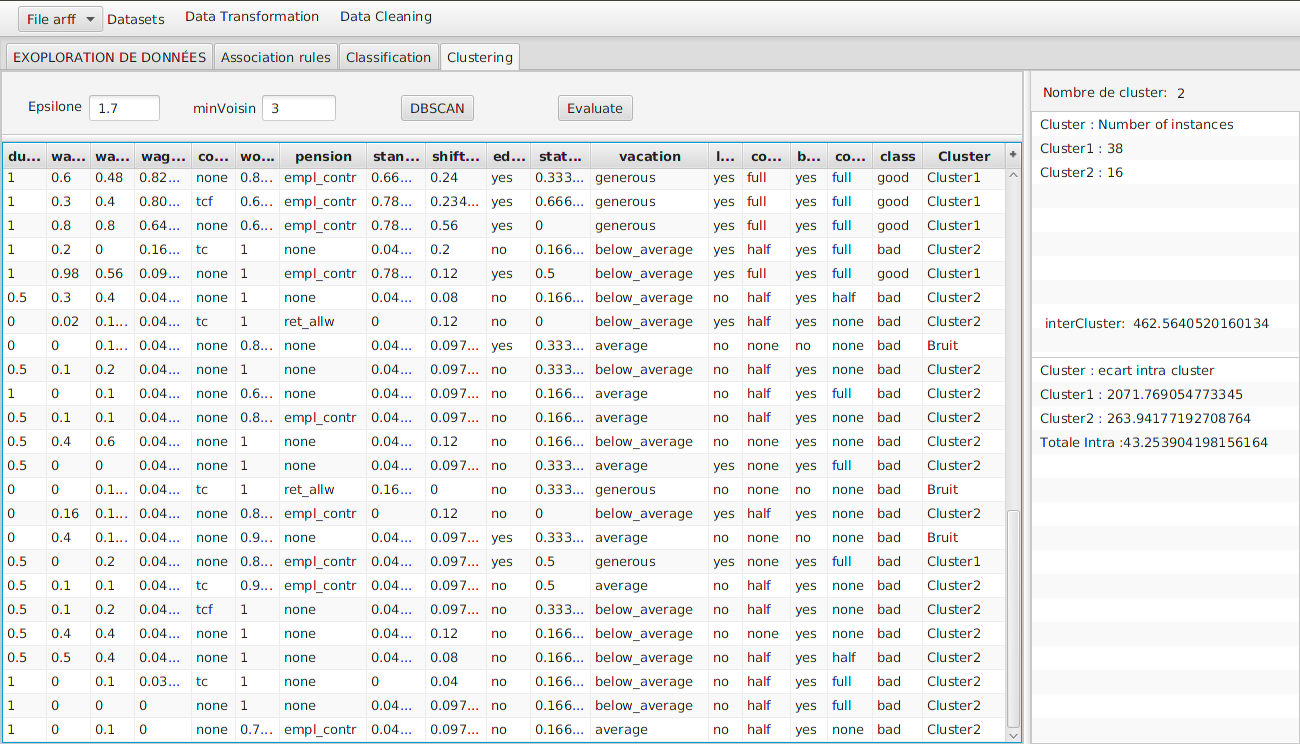
\includegraphics[scale=0.38]{images/dbscan1-2.png}
	\captionof{figure}{Exécution de DBSCAN sur le DataSet LABOR}\label{labelname}%
\end{figure}
\paragraph{Résultats obtenus :}
\begin{itemize}
	\item[$\bullet$] \textbf{2 Clusters: }
	\begin{itemize}
		\item Cluster 1 : 38 instances
		\item Cluster 2 : 16 instances
		\item Bruit : 3 instances
	\end{itemize}
	\item[$\bullet$] \textbf{Inertie:}
	\begin{itemize}
		\item Inter-Cluster : 462.56
		\item Intra-Cluster : 43.25
	\end{itemize}
	\item[$\bullet$] \textbf{Temps d'exécution : 3ms}
\end{itemize}


\subsubsection*{DataSet : IRIS (150 instance/5 attributs)}
\begin{itemize}
	\item[$\bullet$] \textbf{Numérique}
	\item[$\bullet$] \textbf{Epsilon = 0.3}
	\item[$\bullet$] \textbf{MinPts = 7}
\end{itemize}

\begin{figure}[H]
	\centering
	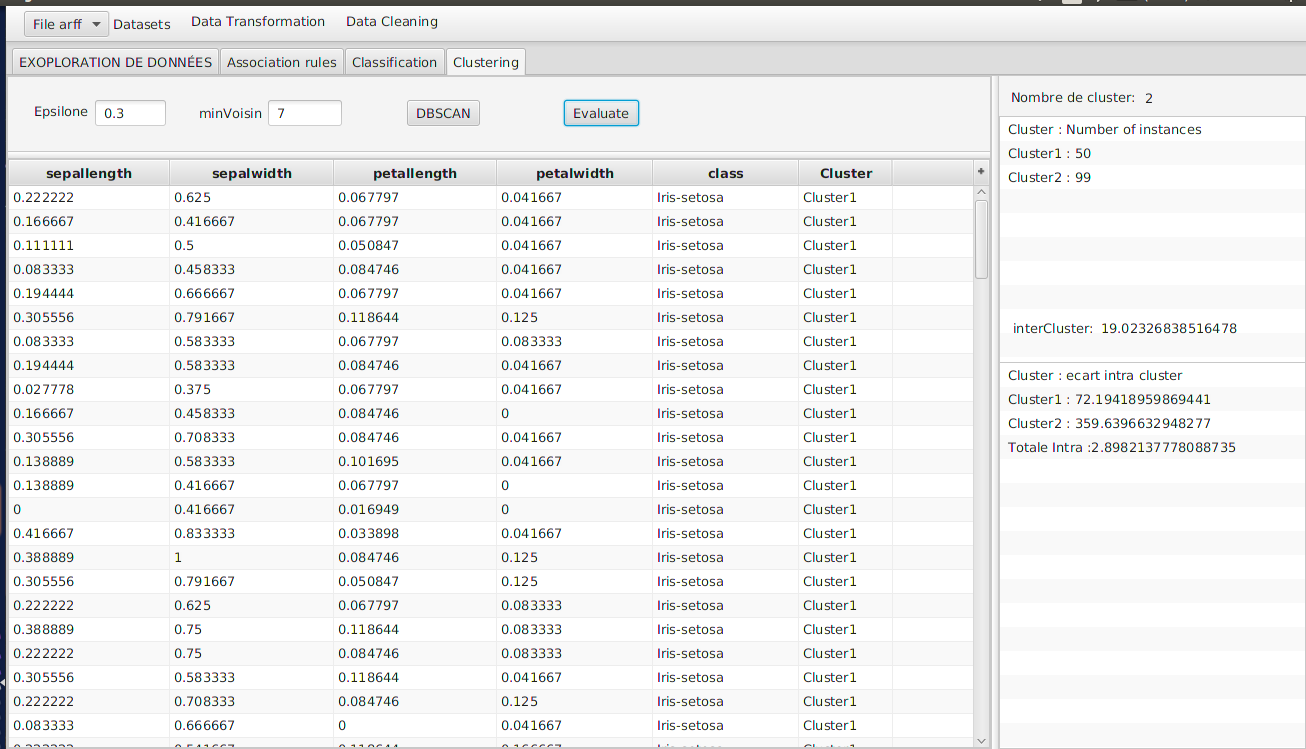
\includegraphics[scale=0.38]{images/dbscan2-2.png}
	\captionof{figure}{Exécution de DBSCAN sur le DataSet IRIS}\label{labelname}%
\end{figure}
\paragraph{Résultats obtenus :}
\begin{itemize}
	\item[$\bullet$] \textbf{2 Clusters: }
	\begin{itemize}
		\item Cluster 1 : 50 instances
		\item Cluster 2 : 99 instances
		\item Bruit : 1 instances
	\end{itemize}
	\item[$\bullet$] \textbf{Inertie:}
	\begin{itemize}
		\item Inter-Cluster : 19.02
		\item Intra-Cluster : 2.89
	\end{itemize}
	\item[$\bullet$] \textbf{Temps d'exécution : 12ms}
\end{itemize}

\subsubsection*{DataSet : GLASS (214 instance/10 attributs)}
\begin{itemize}
	\item[$\bullet$] \textbf{Mixte (Nominal + numérique)}
	\item[$\bullet$] \textbf{Epsilon = 0.3}
	\item[$\bullet$] \textbf{MinPts = 7}
\end{itemize}

\begin{figure}[H]
	\centering
	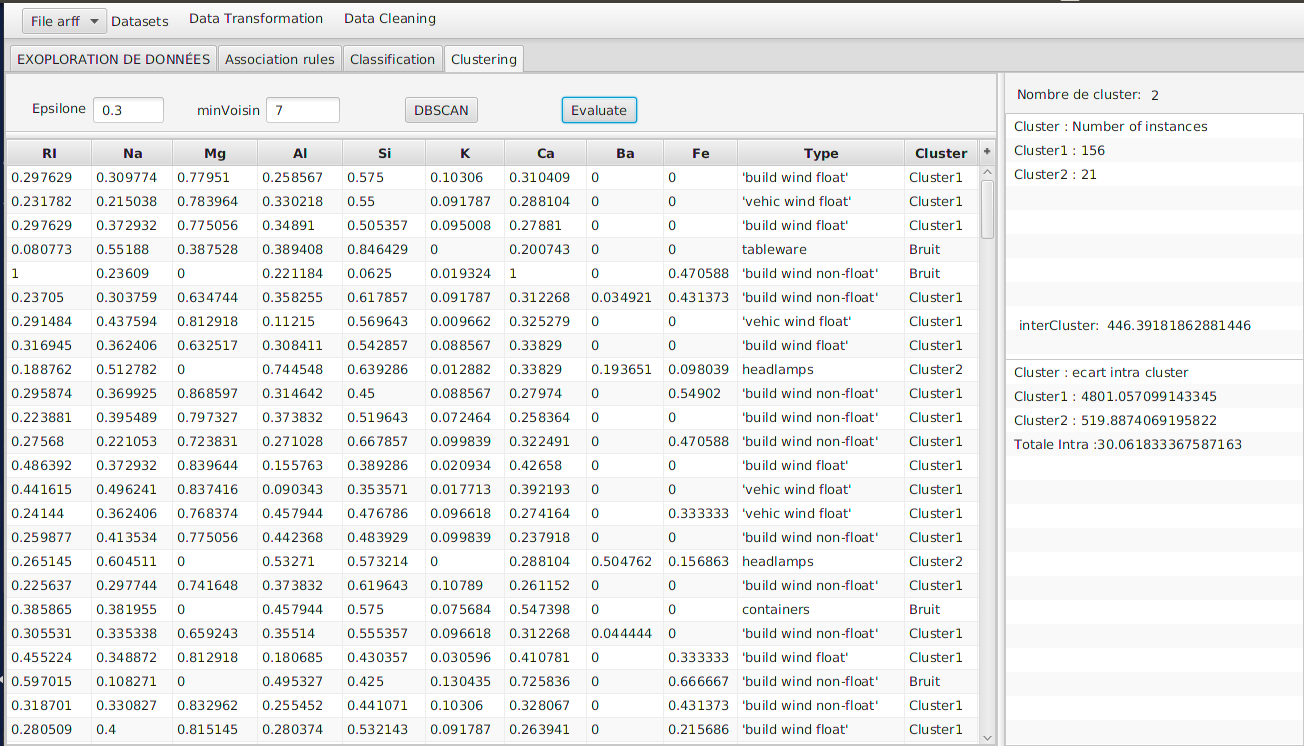
\includegraphics[scale=0.38]{images/dbscan3-2.png}
	\captionof{figure}{Exécution de DBSCAN sur le DataSet GLASS}\label{labelname}%
\end{figure}
\paragraph{Résultats obtenus :}
\begin{itemize}
	\item[$\bullet$] \textbf{2 Clusters: }
	\begin{itemize}
		\item Cluster 1 : 156 instances
		\item Cluster 2 : 21 instances
		\item Bruit : 37 instances
	\end{itemize}
	\item[$\bullet$] \textbf{Inertie:}
	\begin{itemize}
		\item Inter-Cluster : 446039
		\item Intra-Cluster : 30.06
	\end{itemize}
	\item[$\bullet$] \textbf{Temps d'exécution : 24ms}
\end{itemize}



\subsubsection*{DataSet : VOTE (425 instance/17 attributs)}
\begin{itemize}
	\item[$\bullet$] \textbf{Nominal}
	\item[$\bullet$] \textbf{Epsilon = 1.5}
	\item[$\bullet$] \textbf{MinPts = 10}
\end{itemize}

\begin{figure}[H]
	\centering
	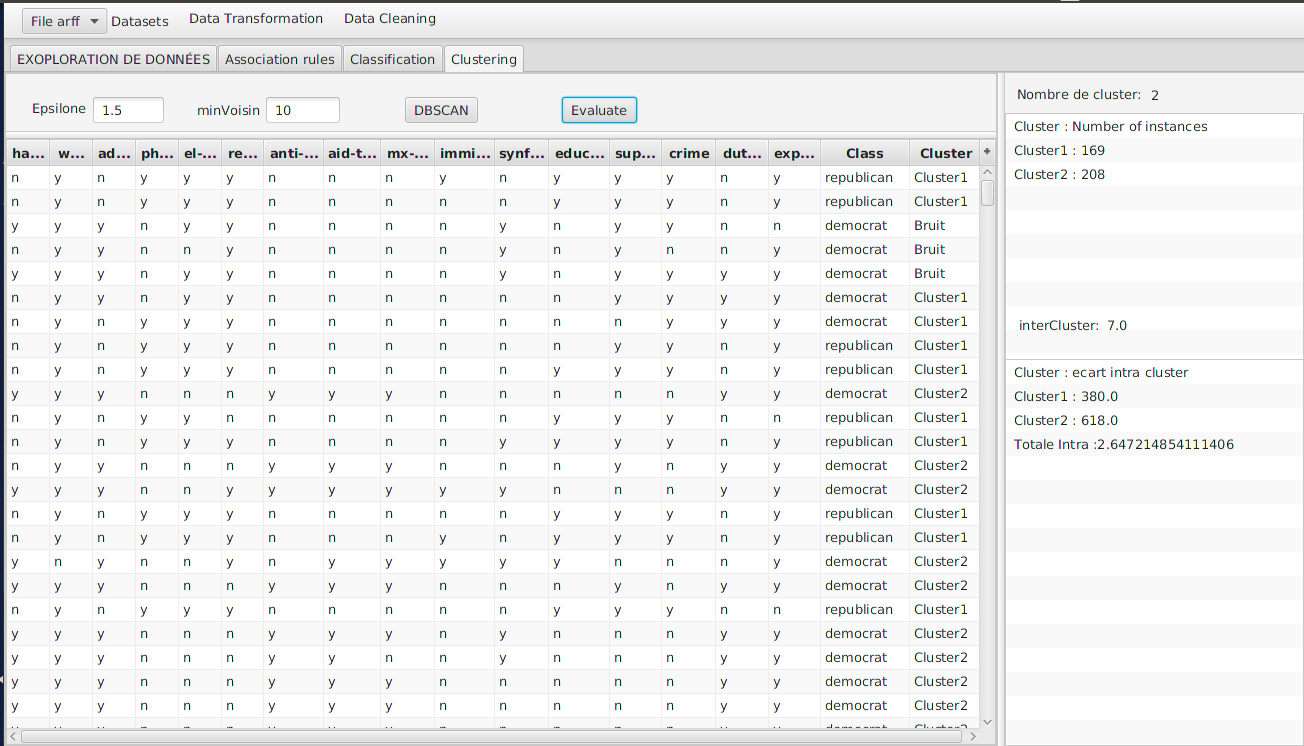
\includegraphics[scale=0.38]{images/dbscan4-2.png}
	\captionof{figure}{Exécution de DBSCAN sur le DataSet VOTE}\label{labelname}%
\end{figure}
\paragraph{Résultats obtenus :}
\begin{itemize}
	\item[$\bullet$] \textbf{2 Clusters: }
	\begin{itemize}
		\item Cluster 1 : 169 instances
		\item Cluster 2 : 208 instances
		\item Bruit : 58 instances
	\end{itemize}
	\item[$\bullet$] \textbf{Inertie:}
	\begin{itemize}
		\item Inter-Cluster : 7
		\item Intra-Cluster : 2.64
	\end{itemize}
	\item[$\bullet$] \textbf{Temps d'exécution : 122ms}
\end{itemize}


\subsubsection*{DataSet : UNBALANCED (856 instance/33 attributs)}
\begin{itemize}
	\item[$\bullet$] \textbf{Numérique}
	\item[$\bullet$] \textbf{Epsilon = 1}
	\item[$\bullet$] \textbf{MinPts = 7}
\end{itemize}

\begin{figure}[H]
	\centering
	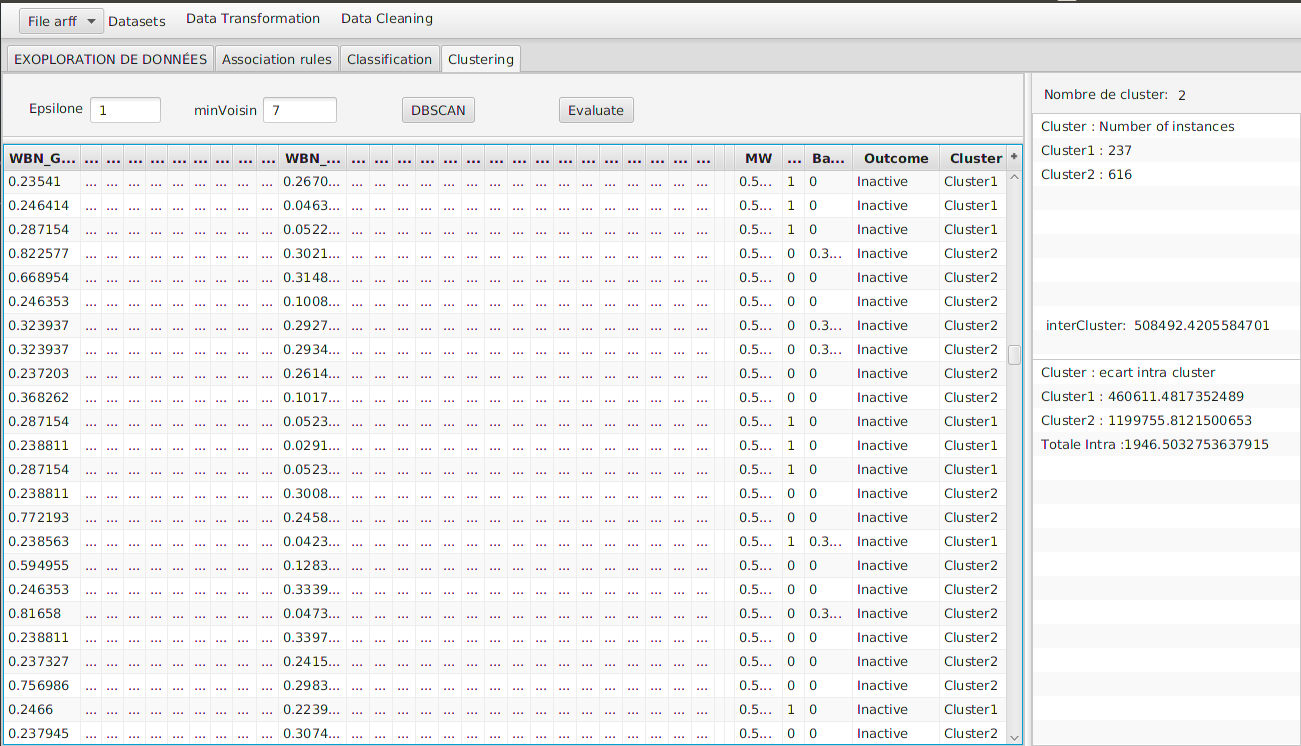
\includegraphics[scale=0.38]{images/dbscan5-2.png}
	\captionof{figure}{Exécution de DBSCAN sur le DataSet UNBALANCED}\label{labelname}%
\end{figure}
\paragraph{Résultats obtenus :}
\begin{itemize}
	\item[$\bullet$] \textbf{2 Clusters: }
	\begin{itemize}
		\item Cluster 1 : 237 instances
		\item Cluster 2 : 616 instances
		\item Bruit : 3 instances
	\end{itemize}
	\item[$\bullet$] \textbf{Inertie:}
	\begin{itemize}
		\item Inter-Cluster : 508492.42
		\item Intra-Cluster : 1946.5
	\end{itemize}
	\item[$\bullet$] \textbf{Temps d'exécution : 779ms}
\end{itemize}


\subsubsection*{récapitulatif des résultats}
Dans le tableau ci-dessous, nous avons regroupé les résultats des expérimentations mentionnées un peu plus haut:
\begin{center}
	\begin{tabular}{|p{2cm}|p{1.2cm}|p{1.2cm}|p{1.5cm}|p{1.5cm}|p{1.5cm}|p{1.5cm}|p{1.5cm}|p{1.2cm}|}
		\hline
		\textbf{DataSet} & \textbf{Epsilon} & \textbf{MinPts} & \textbf{Cluster1} & \textbf{Cluster2} & \textbf{Bruit} & \textbf{Inter} & \textbf{Intra} & \textbf{Temps}
		\\
		\hline
		
		%\newline
		Labor & 1.7 & 3 & 38 & 16 & 3 & 462.56 & 43.25 & 3ms
		\\
		\hline
		
		%\newline
		IRIS & 0.3 & 7 & 50 & 99 & 1 & 19.02 & 2.89 & 12ms
		\\
		\hline
		
		
		%\newline
		Glass & 0.3 & 7 & 156 & 21 & 37 & 446.39 & 30.06 & 24ms
		\\
		\hline
		
		%\newline
		Vote & 1.5 & 10 & 169 & 208 & 58 & 7 & 2.64 & 122ms
		\\
		\hline
		
		
		%\newline
		Unbalanced & 1 & 7 & 237 & 616 & 3 & 508492.42 & 1946.5 & 779ms
		\\
		\hline
	\end{tabular} 
\end{center}

\newpage 

\section{Conclusion}
En conclusion, après implémentation de DBSCAN, et suite à plusieurs expérimentations, nous sommes capables de noter remarques importantes suivantes:\\
\begin{itemize}
	\item[$\bullet$] Un avantage de DBSCAN est que Nous n'avons \textbf{pas besoin} de connaitre à l'avance ni le nombre de clusters (K) ni les centres de ces derniers (centriodes).
	
	\item[$\bullet$] \textbf{Epsilon}($\epsilon$) et \textbf{MinPts} sont des paramètres empiriques qu'il faut bien fixer après maintes expérimentations pour avoir les meilleurs résultats escomptés.
	
	\item[$\bullet$] Nous avons la possibilité d'évaluer notre clustering avec les mesures d'Inertie, et pour cela nous devons obtenir l'inertie \textbf{inter-Cluster} $>>$ \textbf{intra-Clutser}.
	
	Cela est bien visible via les résultats que nous avons obtenus (voir tableau des résultats)
	
	\item[$\bullet$] Il est \textbf{obligatoire} de passer par l'étape 1 qui est le pré-traitement,le nettoyage et l'étude du DataSet (\textbf{Missing-value} et \textbf{normalisation}),
	Aussi si la classe est numérique passer par la \textbf{discrétisation} (voir ANNEXE A ).
	
	\item[$\bullet$] Comme le graphe ci-dessous l'illustre: le temps d'exécution est proportionnel à la taille du dataset (nombre d'instances/ nombre d'attributs), c'est-à-dire, plus le nombre d'instance est grand plus le temps d'exécution sera grand.
	
	\begin{figure}[H]
		\centering
		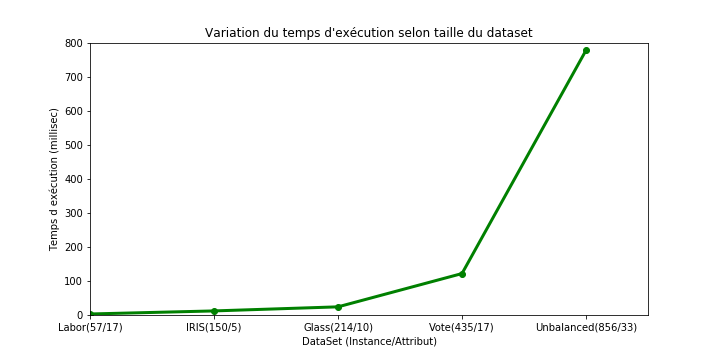
\includegraphics[scale=0.6]{image/dbscanPlot.png}
		\captionof{figure}{Variation du temps d'exécution de DBSCAN selon la taille du DataSet}\label{labelname}%
	\end{figure}
	
	\item[$\bullet$] Le temps d'exécution reste assez réduit même pour de grand DataSets, nous expliquons cela par la complexité de dbscan qui est en \textit{O($n^2$)} comme cité précédemment.
	
	\item[$\bullet$] Les clusters ne correspondent pas forcement à la classe car le clustering étudie les similarités et dissimilarités entre instances.
	
	\item[$\bullet$] Aussi nous avons remarqué que
	le paramètre \textbf{Epsilon} influe sur le nombre de cluster, tel que:  Plus on augmente la valeur d'\textbf{Epsilon} plus il y aura de clusters.\\
	
	Et le paramètre \textbf{MinPts} quant à lui influe sur la densité des clusters, tel que: Plus \textbf{MinPts} sera pris petit plus les cluster seront dense.\\
	
	Ainsi si l'on prend \textbf{Epsilon} assez petit et \textbf{MinPts} assez grand nous obtiendrons plus d'instance classées comme du bruit.\\
	
	
	\item[$\bullet$] On peut exploiter le bruit (outliers) dans des datasets pour un objectif donné, car dbscan arrive à les détecter.\\
\end{itemize}



















\chapter*{Conclusion}
%on va devoir lister tous les points remarquables pour chaque algo  puis comparer entre chaque 2 algo / methodes puis le tous pour dire que chaque methode est spécifique au données qu'on possède et au but de notre projet (pour faire un max de page 3la la conclusion xD)

Suite aux nombreuses expérimentations sur nos  Quatre algorithmes  qui sont :\\

 \textbf{Apriori}, \textbf{Fp-growth}, \textbf{K-nn} et \textbf{Dbscan}\\
 
 Nous avons pu relever plusieurs informations et remarques intéressantes, nous commençons par les deux premiers algorithmes qui concernent:
 
 \paragraph{\underline{l'extraction des items fréquents}}
 sur des dataSets transactionnels généralement , on a pu observer les points suivants sur \textbf{APRIORI}:

\begin{itemize}
	\item Très simple à implémenter  et à comprendre 
	\item Face à grandes instances ( dataset de plus de 200 transactions) il devient très long et prend beaucoup de temps à s'exécuter ( sur nos machines) ceci est en relation direct avec le calcul intensif qu'apriori fait et qui fait sa signature qui est la jointure à chaque étape pour le calcul les itemset candidats, puis il repasse encore sur le dataset transactionnel pour calculer le support de chaque itemset candidats afin de filtrer ses derniers ceci augmente la complexité d'apriori et le rend ainsi Long.
	\item Efficace  il arrive au résultat avec une bonne précision c'est à dire qu'il extrait exactement tous les items fréquents. 
\end{itemize}

Il existe des versions d'apriori qui sont plus rapide et qui ont proposé une solution à sa lenteur comme :

 Pour la jointure on code les itemset sur un tableau de taille des items on mettra 0 quand l'item n'apparait pas dans l'itemset et 1 sinon ainsi on pourra remplacer la jointure par :
\begin{itemize}
	\item l'opérateur OU logique .(exemple : soit un dataset ayant que trois items distincts et deux items set de longeur deux un exemple de jointure entre les deux sera comme suit :$[i_{1}:0,i_{2}:1,i_{3}:1] OU [i_{1}:1,i_{2}:1,i_{3}:0] = [i_{1}:1,i_{2}:1,i_{3}:1]$)
\end{itemize}

Représentation du dataset verticalement ( principe de la recherche d'information fichier inverse)  c'est à dire pour chaque item va pointer vers un tableau de taille des transactions on mettera un 0 quand l'item n'apparaît pas dans la case de la transaction et 1  sinon ainsi pour le calcul de support d'un item set on fera un ET logique qui sera comme suit:
\begin{itemize}
	\item l'opérateur Et logique .(exemple : soit un dataset ayant que trois Transactions distincts et deux items set de longueur deux un exemple de jointure entre les deux sera comme suit :$[t_{1}:0,t_{2}:1,t_{3}:1] ET [t_{1}:1,t_{2}:1,t_{3}:0] = [t_{1}:0,t_{2}:1,t_{3}:0]$) le support de l'itemset sera le nombre de 1 .
\end{itemize}

Ceci réduit considérablement le temps d'exécution .
mais il existe un autre algorithme proposé par Han FP-growth dans lequel il s'est intéressé à une modélisation et implémentation complètement différente en exploitant les arbres.

Plus Concrètement, \textbf{FP-GROWTH} utilise de tout autres structures de données, il s'agit d'une représentation compressée du Dataset sous forme d'arbre (FP-Tree), ainsi sa construction ne nécessite que 2 scans du DataSet, puis la suite de l'exécution se fait en accédant uniquement au FP-Tree. Soient les points suivants nos principales remarques à ce sujet:
\begin{itemize}
	\item Implémentation plus compliqué.
	\item Nette réduction du temps d'exécution par rapport à Apriori, même pour de grandes instances (DataSet) les temps d'exécution restent très raisonnables.
	\item C'est aussi un algorithme complet car il arrive toujours a extraire tous les items fréquents. 
\end{itemize}


\paragraph{\underline{Classification supervisée et non supervisée}}

Dans ce projet on eu affaire à deux  algorithmes de classification :
\begin{itemize}
	\item \textbf{K nearest neighbors} "K plus proche voisins" dans la classe des algorithmes de classification supervisé
	\item \textbf{DBscan} dans la classe des algorithmes de classification non supervisé 
\end{itemize}
 
\paragraph{ Dans la classification avec K-NN on peut noter les points essentiels suivants:}
 \begin{itemize}
 	\item L'étape du prétraitement est primordiale pour une bonne précision.
 	\item c'est un algorithme de classification sensible au bruit principalement si on prend par exemple un nombre de voisin assez petit par exemple trois voisins et deux de ces voisins sont des bruits "mal classifié" on va alors classifier notre instance avec la mauvaise classe .
 	\item K NN  se base sur un principe simple ( similarité ) donc le choix des fonctions de distances  influencera de manière considérable la classification .
 	\item les données d'entraînement doivent couvrir toutes les classes potentiels et doivent être assez diverse ce qui implique plusieurs instances pour une classe sinon K nn sera incapable de  prédire la classe de l'instance à classifier dans les données de testes car la classe n'existe pas dans les données d'entraînement.
 	\item le temps d'exécution augmente de façon exponentielle quand nos données d'entraînements et de testes dépasse les 1000 instances , on peut expliquer ça par le fait que pour avoir les plus proches voisins on est obligé de passer par le tri ( complexité quadratique) qui ralentit  le processus de classification , ainsi que le calcul de distances entre l'instance à classifier et toutes les données d'entraînements.
 	\item K est un paramètre empirique qu'il faut fixer lors des expérimentations pour une bonne classification choisir et qui dépend directement du nombre de classe de nos données  à classifier .
 	
 \end{itemize}
 
 
\textbf{Des améliorations} par contre peuvent être suggérées comme :

On pourrait éviter le tri après le calcul de distances et utiliser à la place une liste de taille K triée généralement K n'est pas très grands  comparer  à la taille des données ,ainsi à chaque calcul de distance de l'instance avec les données d'entraînements:
\begin{enumerate}
	\item  si la distance qu'on est entrain de calculer 
	est supérieur à toutes les instances de la liste alors on l'ajoute , on pourra comparer toujours avec le dernier car notre liste est triée (de k éléments).
	\item sinon
	alors cette instance doit être ajouté en la remplaçant avec celle qui lui est ai supérieur en utilisant une fonction d'insertion dans une liste triée .
	
	
\end{enumerate}  

\paragraph{Dans le clustering avec DBSCAN nous avons constaté les points suivants:}
\begin{itemize}
	\item L'étape du pré-traitement (aussi bien le traitement des valeurs manquantes que la normalisation) est NON négligeable pour une bonne précision, sachant que la distance Epsilon  dépend directement de la normalisation.
	
	\item Contrairement aux algorithmes de classification supervisée nous n'avons pas le nombre de cluster/class au préalable, ce qui permet de réellement clusteriser selon les similitudes et dissimilitudes des objets/instances.
	
	\item Par contre, pour DBSCAN étant basé densité nous avons 2 paramètres à fixer après expérimentation, qui sont Epsilon et MinPts,ceux là permettent de décider de la densité (concentration) des objets/instance dans les clusters.
	
	\item  DBSCAN étant simple à implémenter, a en plus la particularité de ne pas être couteux en temps d'exécution, vu sa complexité.
	
	\item Cet algorithme est tout aussi efficace dans la détection d'outlier, car certaines études s'intéressent justement au valeurs aberrantes, ainsi Dbscan permet leur extraction.
	
	\item Le paramètre Epsilon étant une mesure de distance, dbscan tout comme K-nn dépend de la fonction de mesure de distance utilisée (euclidienne,manathan, ..)
\end{itemize} 

\textbf{Certaines améliorations} peuvent être suggérées:

Il est à noter que les objets/instances d'un dataset n'ont pas tous la même densité, ainsi il se peut qu'en choisissant des valeurs de Epsilon et MinPts trop petites, certain clusters soient bien formés et d'autres absolument pas, ou meme que beaucoup d'instances soient classées comme bruit sans l'être.
\begin{itemize}
	\item C'est pour cela qu'un solution serais de seuiller ses deux paramètres, par exemple avec un Min-Epsilon et Max-Epsilon, de même pour le nombre de voisins: Min-Pts et Max-Pts.
\end{itemize}

\newpage 
\paragraph{\underline{Comparons les trois catégories de techniques:}}
Les 3 catégories d'algorithme de Data-Mining vu au cours de ce projet sont chacune spécifique à une catégorie de problème, tel que:
\begin{itemize}
	\item Pour l'étude des motifs fréquents, des associations courantes des attributs d'un dataset, ou l'étude de dataset transactionnel, nous utilisons la $1^ere$ catégorie qui regroupe: \textbf{Apriori} et \textbf{FP-Growth}.
	
	\item Pour la classification d'objets/Instances dont on a connaissance des classes que nous souhaitons obtenir, et que nous avons à disposition des datasets de training, nous avons plus intérêt à utiliser les algorithmes de classification supervisées dont \textbf{K-NN}.
	
	\item Pour l'étude des similitudes et dissimilitudes entre objets/Instances, la détection d'outliers, ou la classification mais que nous ne possédons pas de dataset de training, nous nous dirigerons alors aux algorithmes de classification non-supérvisées (clustering) dont \textbf{DBSCAN}.
\end{itemize}

Ainsi nous concluons que chaque problème possède des méthodes / techniques qui lui sont le plus appropriées, c'est pour quoi il faut avoir connaissance de l'ensemble du problème sous tous ses aspects pour savoir vers quelles techniques se diriger, cependant dans une même catégorie il existe plusieurs algorithmes, qu'ils faut maitriser afin de choisir le plus adéquat selon les avantages et inconvénients de chacun.

\newpage

\chapter*{ANNEXE A}
Nettoyage et traitement du dataset avant clustering:n\\
(DataSet : Unbalanced : Missing-value + Normalisation)
\begin{figure}[H]
	\centering
	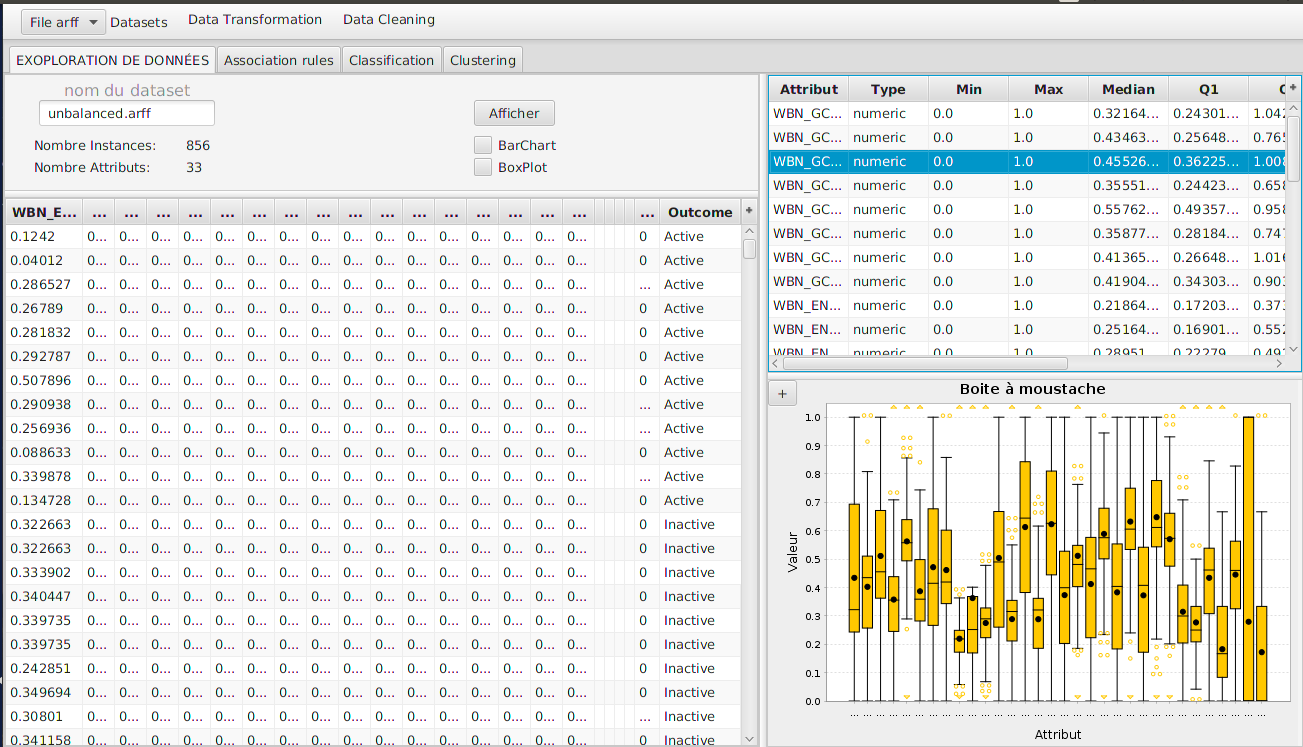
\includegraphics[scale=0.38]{images/dbscan5-1.png}
	\captionof{figure}{Nettoyage et traitement du dataset avant clustering}\label{labelname}%
\end{figure}

\newpage
\chapter*{Références bibliographiques}
\textbf{ }\\

\textbf{[1]} : 
http://www.cs.ccsu.edu/~markov/ccsu\_courses/DataMining-1.html
\textbf{ }\\

\textbf{[2]} : Han's book : DataMining conceptis and technique third edition Morgan kaufmann.\\
\textbf{ }\\

\textbf{[3]} : https://fr.slideshare.net/ssuserab1db8/les-algorithmes-de-gnration-des-rgles-d-association\\
\textbf{ }\\

\textbf{[4]} : https://archive.ics.uci.edu/ml/datasets/Online+Retail



\end{document}


